\documentclass{article}
\usepackage{amsmath}
\usepackage{breqn}
\usepackage{amssymb}
\usepackage{dirtree}

\usepackage{algorithm}
\usepackage[noend]{algpseudocode}


\usepackage{geometry}
\geometry{margin=1in}

\usepackage{hyperref}
\hypersetup{
    colorlinks=true,
    linkcolor=black,
    urlcolor=cyan,
}

\usepackage{wrapfig}
\usepackage{graphicx}

\usepackage{array}
\graphicspath{ {./images/} }

\setcounter{secnumdepth}{4}
\setcounter{tocdepth}{2}

\usepackage{xcolor,soul,lipsum}

\makeatletter
\newcommand\subsubsubsection{\@startsection{paragraph}{4}{\z@}{-2.5ex\@plus -1ex \@minus -.25ex}{1.25ex \@plus .25ex}{\normalfont\normalsize\bfseries}}
\newcommand\subsubsubsubsection{\@startsection{subparagraph}{5}{\z@}{-2.5ex\@plus -1ex \@minus -.25ex}{1.25ex \@plus .25ex}{\normalfont\normalsize\bfseries}}
\newcommand\subsubsubsubsubsection{\@startsection{subparagraph}{6}{\z@}{-2.5ex\@plus -1ex \@minus -.25ex}{1.25ex \@plus .25ex}{\normalfont\normalsize}}
\newcommand{\myhy}[2]{\hyperref[#1]{\color{black}\setulcolor{black}\ul{#2}}}
\makeatother


\begin{document}
\begin{titlepage}
    \begin{center}
        \vspace*{1cm}
            
        \Huge
        \textbf{Playing checkers using reinforcement learning}
            
        \vspace{0.5cm}
        \LARGE
        An investigation into playing checkers using a reinforcement learning via a neural network library, with an implementation of
        automatic differentiation, built from scratch.

        TODO: 2.3.3 ONWARDS
            
        \vspace{1.5cm}
            
        \textbf{Edgar Maddocks}            
        \vfill
            
        \vspace{0.8cm}
                        
        \Large
        Bedford School\\
        03/05/2024\\
            
    \end{center}
\end{titlepage}

    \pagebreak

    \tableofcontents

    \section{Analysis}
    \subsection{Background}
    This project is an investigation into the use of reinforcement learning to play games (in this case checkers/checkers).
    The model will use self-play and Monte Carlo tree search algorithms, coupled with a multi-headed neural network to
    understand the game and estimate optimal actions.

    The neural network will be built using a library, that has an autograd engine implemented, all built from scratch. This
    investigation will however use some scientific computing libraries for faster simple matrix operations (such as numpy). Some more
    complex functions (such as cross-correlation and its derivative) will also be built from scratch.

    \pagebreak
    \subsection{Evidence of Analysis}

    \subsubsection{Current systems}

    \subsubsubsection{Checkers} \label{checkers}
    checkers is an English board game played on an 8x8 checkered board, identical to a chessboard.
    Each player begins a game with 12 pieces, usually flat round discs.
    The pieces and board are usually black and white, and will be referred to as such.
    The board is first placed between the two players such that the bottom right-hand corner is a white square,
    for both players.
    
    A coin is tossed to decide who plays black, and that player has the first move. Each player places their pieces
    on the 12 black squares closest to themselves. The setup of the board can be seen in Figure 1. 

    \begin{wrapfigure}[15]{l}{0.3\linewidth}
        \centering
        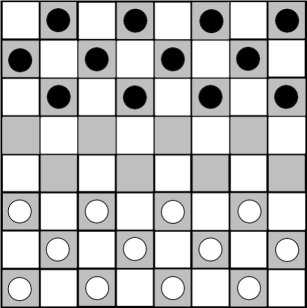
\includegraphics[scale=0.35]{The-starting-position-for-checkers.png}
        \caption{An image showing the starting position of a game of checkers}
    \end{wrapfigure}
    The pieces only move diagonally (so will always be on black squares)
    and the aim is to take all of the opposing players pieces, or to put the opposing player in a position with no possible moves.
    Players take turns moving their shade of pieces. If at any point of the game, a player's piece reaches the opposing players edge
    of the board, the piece becomes a 'King', and another piece should be placed on top of said piece to indicate so.
    Unless a piece is crowned and a 'King' it may only move and take pieces diagonally forwards. Kings may move and take both forwards and backwards.
    
    \begin{wrapfigure}[12]{r}{0.5\linewidth}
        \centering
        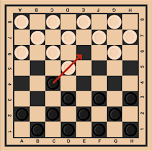
\includegraphics[scale=1.15]{piece being taken.png}
        \caption{Example of a piece being taken in checkers}
    \end{wrapfigure}
    If an adjacent square has an opponents piece and the square immediately beyond the oppositions piece is empty, the opponents piece may be captured.
    If the player whose go it is, has the opportunity to capture one or more pieces, then they must do so. 
    A piece is taken by moving your own piece over the opposing player's, into the vacant square, and then removing the opposing piece from the board.
    An example of this process can be seen in Figure 3.

    Unlike a regular move, a capturing move may make more than one 'hop'. This is if the capture places the piece in a position where another capture is possible.
    In this case, the additional capture must be made. The capture sequence can only be made by one piece per move. i.e. You cannot make one capture with one piece, 
    and then another capture with another piece in the same move.
    
    However, if more than one piece can capture, the player has free choice over which piece to move. Likewise, if one piece can capture in multiple
    directions then the player has the choice in which direction to move. 
    
    
    \textbf{Note:} it is not compulsory for the player to move in the direction, or with the piece,
    that will lead to the greatest number of captures in that move.
    
    \begin{figure}[h]
        \centering
        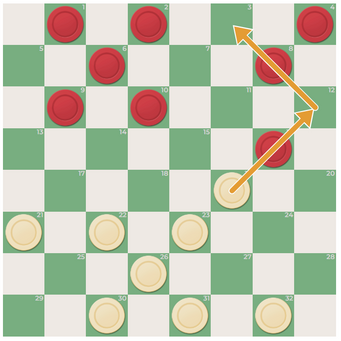
\includegraphics[scale=0.6]{double hop.png}
        \caption{Visualization of multiple captures in one move}
    \end{figure}

    A move may only end when the position has no more captures available or an uncrowned piece becomes a King. 
    The game ends when all of a players piece's have been captured, or a player has no available moves.

    \pagebreak
    \subsubsubsection{Neural Networks}
    \subsubsubsubsection{What is a neural Network}
    A neural network is a machine learning model which aims to mimic the processes of the human brain.
    Each network contains inputs and outputs, as well as one or more layers of hidden nodes - which act as artificial neurons.

    Neural networks are a supervised learning model, meaning that they learn from labeled data (which has the objective correct answer in the data).
    They are sometimes referred to as artificial neural networks (ANNs) or simulated neural networks (SNNs).\\

    In a fully connected network, each node is connected once to each node in the next layer - an example of how one node connects
    to the next layer can be seen below.
    \begin{figure}[h]
        \centering
        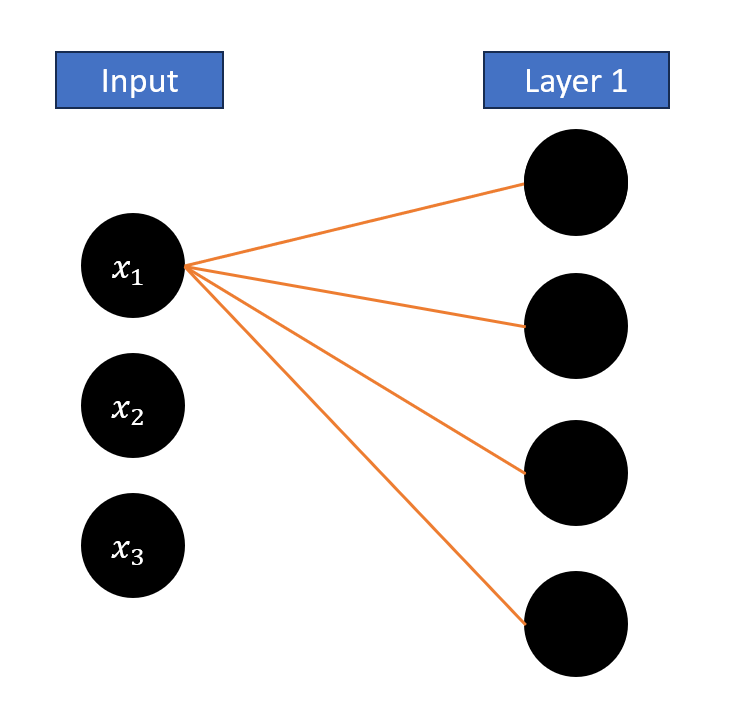
\includegraphics[scale=0.2]{ConnectedNode.png}
        \caption{Example of a fully connected node and layer}
    \end{figure}

    Neural networks can be modelled as a collection linear regression units.

    \subsubsubsubsection{Linear Regression Unit}
    A single linear regression unit output has the formula:
    \begin{align}
        \hat{y} = \sum_{i=0}^{n} w_ix_i + b
    \end{align}

    Where $\hat{y}$ is the predicted output, $n$ is the number of inputs, $x_i$ is the $i$th input, $w_i$ is the weight of $x_i$, and $b$ is a bias.
    If, for example, there were 3 inputs the full equation for $\hat{y}$ would be:
    \begin{align}
        \hat{y} = w_1x_1 + w_2x_2 + w_3x_3 + b
    \end{align}

    \subsubsubsubsection{Vectorization of processes}
    This calculation can be vectorized to improve efficiency and would be notated:
    \begin{align}
        \hat{y} = XW + b
    \end{align}

    Where we let
    \begin{align}
        W = \begin{bmatrix}
            w_1\\
            w_2\\
            \vdots\\
            w_n
        \end{bmatrix}\\
        \hspace{25px}
        X = \begin{bmatrix}
            x_1&
            x_2&
            \hdots&
            x_n
        \end{bmatrix}
    \end{align}

    $X$ here is a row vector as this is the most common format for data as an input to a network (e.g. being read from a csv).
    This parallelized computation is much faster, and can be parallelized using the GPU to further improve speed and efficiency.

    \subsubsubsubsection{Forward Pass of Dense Layer}
    In the case of neural networks, lots of these linear regression units can be combined to form a vector of outputs.
    Each of these regression units will have the same inputs, therefore $X$ can have the same definition. However, $W$ will now be
    composed of multiple vectors of weights, instead of just one.

    Here we let
    \begin{align}
        W = \begin{bmatrix}
            w_{11} & w_{21} & \dots & w_{j1}\\
            w_{12} & w_{22} & \dots & w_{j2}\\
            \vdots & \vdots & \ddots & \vdots\\
            w_{1n} & w_{2n} & \dots & w_{jn}
        \end{bmatrix}
    \end{align}

    Where $j$ is now the number of nodes in the layer. If we rewrite our forward pass equation to use this weight matrix,
    with each node as its own regression unit:
    \begin{align}
        Y = XW + B
    \end{align}

    Where:
    \begin{align}
        Y = \begin{bmatrix}
            \hat{y_1}&
            \hat{y_2}&
            \hdots&
            \hat{y_n}
        \end{bmatrix} \hspace{15mm}
        B = \begin{bmatrix}
           b_1 & b_2 & \dots & b_j
        \end{bmatrix}
    \end{align}

    With $W$ and $X$ having the same definition as most recently defined.

    \subsubsubsubsection{Forward Pass of a Convolutional Layer}
    The main function of a convolutional layer is to extract key features and they are often used in image recognition and classification solutions.

    \begin{wrapfigure}[15]{r}{0.5\linewidth}
        \centering
        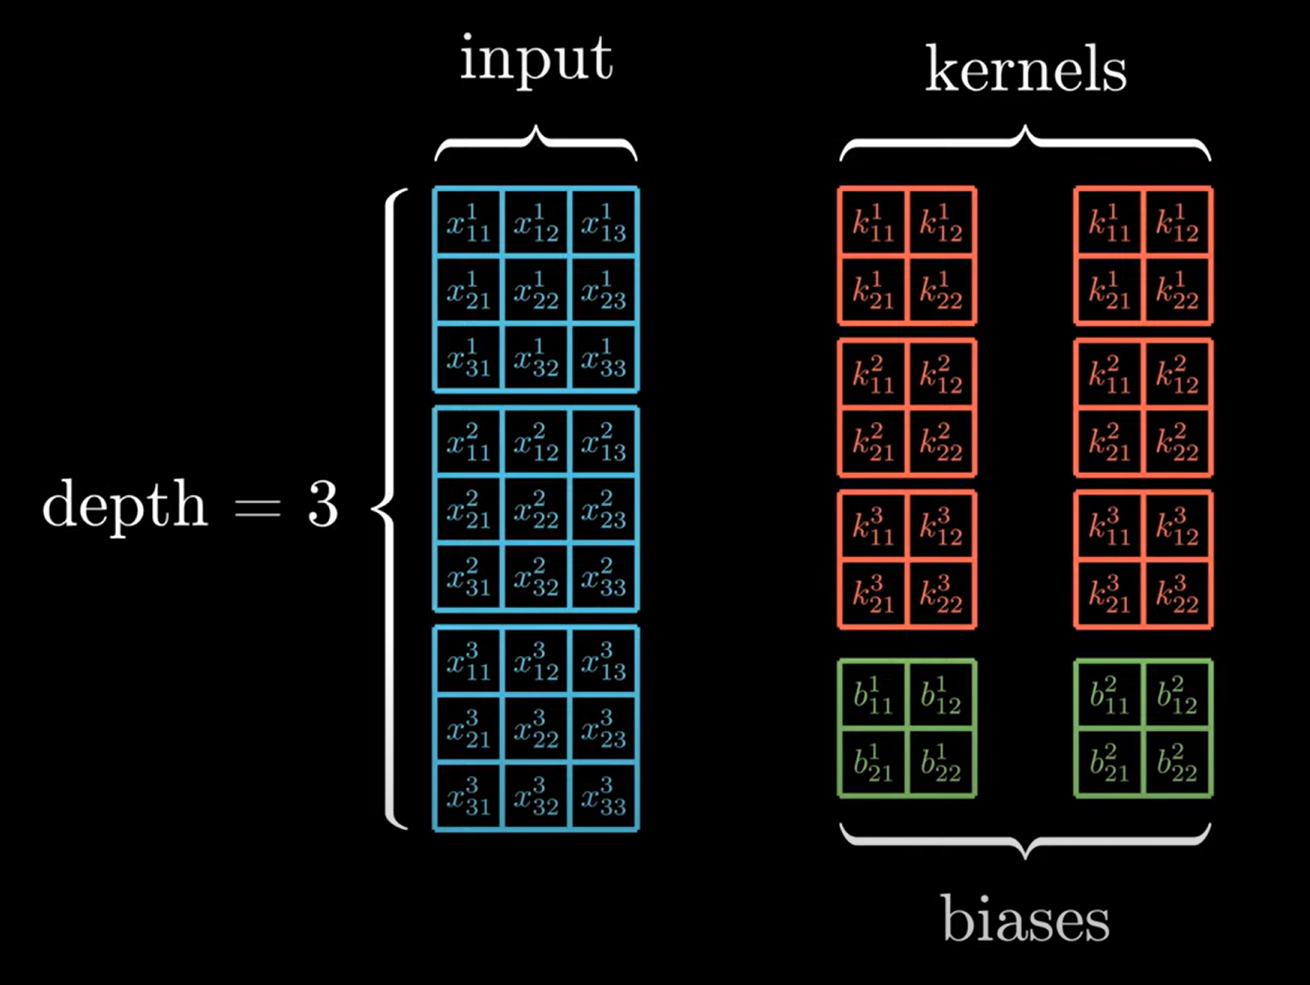
\includegraphics[scale=0.2]{ConvInputIndependentCode.png}
        \caption{Visualization of a Convolutional layer}
    \end{wrapfigure}

    A convolutional layer takes in a 3 dimensional block of data. This can be imagined as the first 2 dimensions being a grid of pixels, and the third dimension
    being the colour channels for each grid. The trainable parameters in a convolutional network are the kernels/filters and the biases. The kernels can be of any size
    but must have the same depth as the input data. Each kernel also has a bias matrix, which has the same shape as the output.

    After the forward pass, the output will also be 3 dimensional, but here the depth is equal to the number of kernels, and the size is equal to

    \begin{align}
        I - K + 1
    \end{align}

    Where $I$ is the size of the input grid and $K$ is the size of the kernel grids.

    The forward pass can then be simplified, with each output equating to the bias for that kernel plus the sum of the sum of cross correlations between a single channel
    of the input and its respective channel in the kernel. This can be seen in the figure below, where $d$ is equal to the number of kernels, and $n$ is the number of channels in the input data.


    \pagebreak
    \begin{figure}
        \centering
        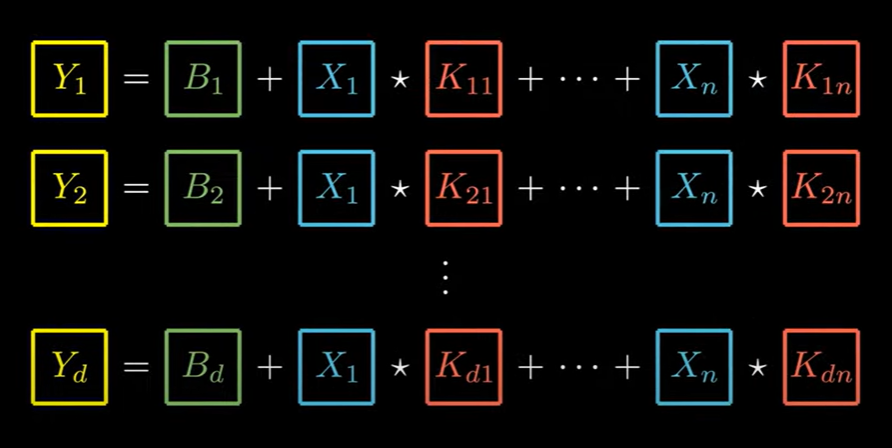
\includegraphics[scale=0.3]{ConvForwardPropIndependentCode.png}
        \caption{Representation of the forward pass of a convolutional layer}
    \end{figure}

    This can be written more mathematically using a summation.

    \begin{align}
        Y_i = B_i + \sum_{j=1}^{n}X_j \star K_{ij}, \hspace{1cm} i = 1 \dots d
    \end{align}

    \subsubsubsubsection{Gradient Descent} \label{Analysis-GradientDescent}

    Now, to update the weights of our model, we can compute these values in closed form, however, it comes with a large time complexity (greater than $O(n^3)$), and therefore
    a process called gradient descent is usually employed.

    Gradient descent works to minimize the error of a model by iteratively locating a minimum in the error function.
    For example, a common cost (error) function is mean squared error.
    \begin{align}
        MSE(Y, \hat{Y}) = \frac{1}{n}\sum_{i=0}^{n}\left(y_i - \hat{y}_i\right)^2
    \end{align}

    This function effectively calculates the absolute distance between the predicted value of one data point ($\hat{y_i}$) and the true value at that same point ($y_i$),
    for every value in the dataset (of size $n$) and takes the mean of these distances.
    Again, this calculation can be vectorized using the equation below.
    \begin{align}
        MSE(Y, \hat{Y}) = \frac{1}{n}((Y - \hat{Y})^T \cdot (Y - \hat{Y}))
    \end{align}

    If we plot the MSE curve of different weights and biases - of a single regression unit, it looks as follows.
    \begin{figure}[h]
        \centering
        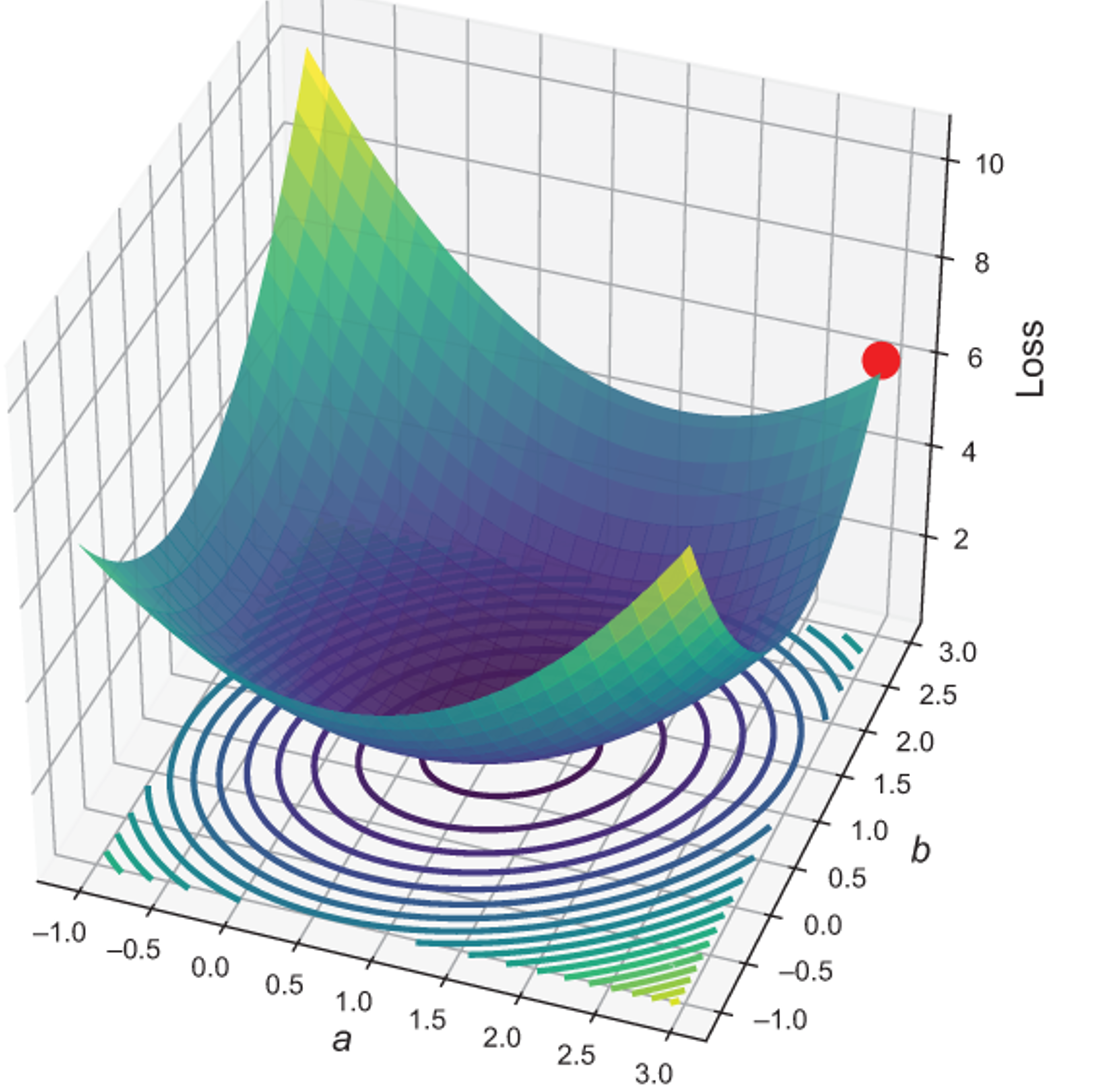
\includegraphics[scale=0.5]{MSEplot.png}
        \caption{Plot of MSE in a single regression unit}
    \end{figure}

    Here the weight has been labelled $a$, but the bias has remained as $b$. As we can see, there is a clear local minimum of this error function,
    and the values that obtain this minimum, is what gradient descent aims to achieve. 
    
    \begin{wrapfigure}[14]{l}{0.4\linewidth}
        \centering
        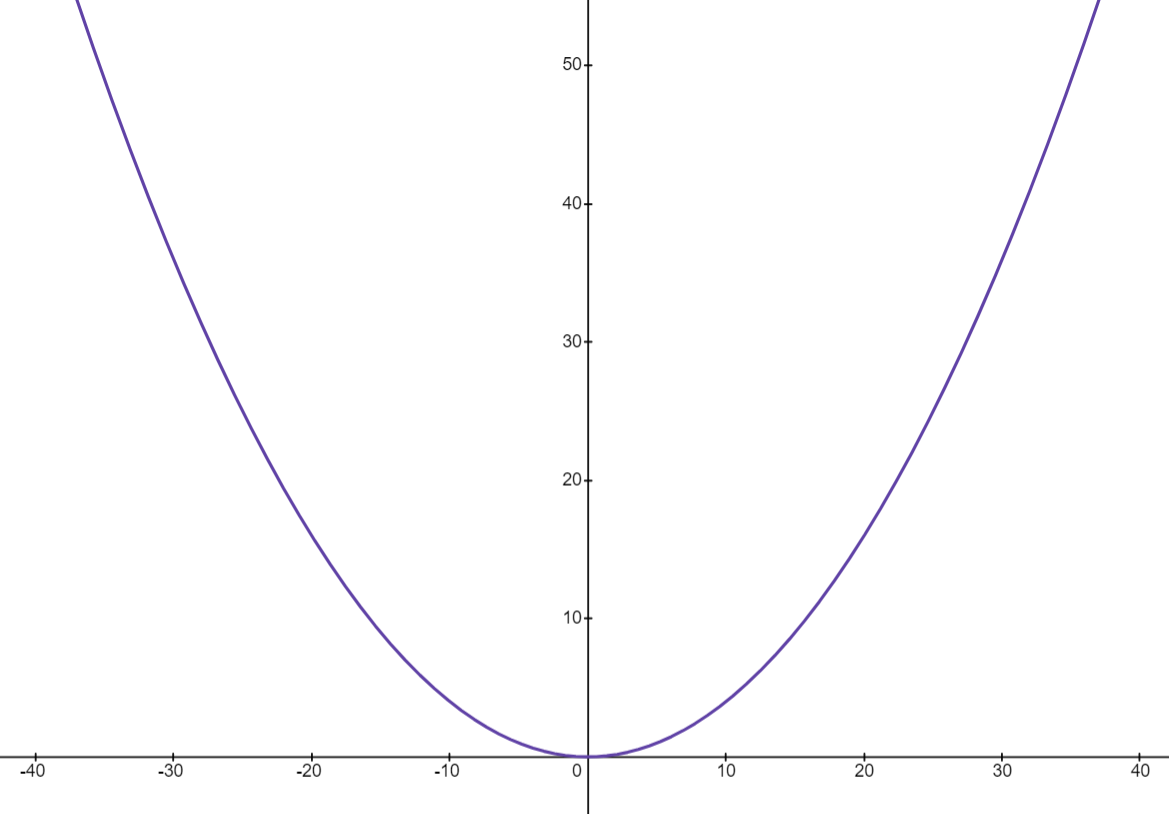
\includegraphics[scale=0.2]{image.png}
        \caption{MSE with respect to one parameter}
    \end{wrapfigure}
    In figure 6 we can see a representation of the MSE plot with respect to only one of the parameters. This makes understanding the process of gradient
    descent much simpler. For example, the minimum of this function ($f(x) = \frac{x^2}{25}$) is at $x = 0$. So, if we were to have an initial $x$ value of say $-40$,
    and we calculated the gradient to be $3.2$, we could then subtract this from $40$. Resulting in a new value of $36.8$, which is closer to our optimal value of $0$.
    This process is completed iteratively until the minimum, or near to it, is reached.

    To denote this mathematically, we can say that 
    \begin{align}
        w_{t+1} = w_t - \alpha \frac{\partial E}{\partial w}\\
        b_{t+1} = b_t - \alpha \frac{\partial E}{\partial b}
    \end{align}

    Where $w_{t+1}$ and $b_{t+1}$ are the parameters at the next timestep, $w_t$ and $b_t$ is the value of the parameters at the current timestep, 
    $\frac{\partial E}{\partial w}$ and $\frac{\partial E}{\partial b}$ are the derivatives of the error with respect to each parameter, 
    and $\alpha$ is the learning rate. This learning rate controls the size of our 'jumps' and prevents the process from beginning to spiral away
    from the optimal values.

    That is a basic overview of gradient descent in a single regression unit, but in a dense network, the process is almost identical. An error function is evaluated, 
    the derivative with respect to the inputs calculated, and the new values updated. The main expense computation-wise is calculating all the derivatives, with respect to
    each set of parameters, as this requires passing the output from the error function backwards through all the layers and processes. To combat this, automatic differentiation
    can be used, which tracks computation dynamically at run time to compute derivatives.

    \subsubsubsection{Automatic Differentiation} \label{Autodiff-example}
    As mentioned, automatic differentiation tracks computation dynamically and then computes derivatives using a computational graph. This allows models to
    have much more complex forward passes, including decision branches and loops where the length of the loop is decided at runtime.

    Automatic differentiation operates by differentiating a complex function (that we don't know the derivative of), by treating it as a composition of more elementary functions
    (of which we do know the derivatives). Additionally, it treats each of these elementary functions as though their output is an intermediate variable when computing the
    complex function. This becomes very useful when there are multiple inputs to the function, and we only want the derivative to one of these variables. Finally, this process
    makes use of the chain rule to compute the derivative with respect to the inputs, as will be shown later on.

    Firstly, I will walk through an example of the process of automatic differentiation.\\
    \noindent Say we have a function: \begin{align}
        f(x) = ln\left(\frac{sin(x_1)}{cos(x_2)}\right)
    \end{align}

    This function has two arbitrary inputs (perhaps in the case of a neural network these could be our parameters or outputs for example). At first, this is quite a complex
    function to differentiate but, we can simplify it using intermediate variables. For example \begin{align}
        v_1 &= sin(x_1)\\
        v_2 &= cos(x_2)\\
        v_3 &= \frac{v_1}{v_2}\\
        v_4 &= ln(v_3)\\
        y &= v_4
    \end{align}

    \begin{wrapfigure}[23]{l}{0.5\linewidth}
        \centering
        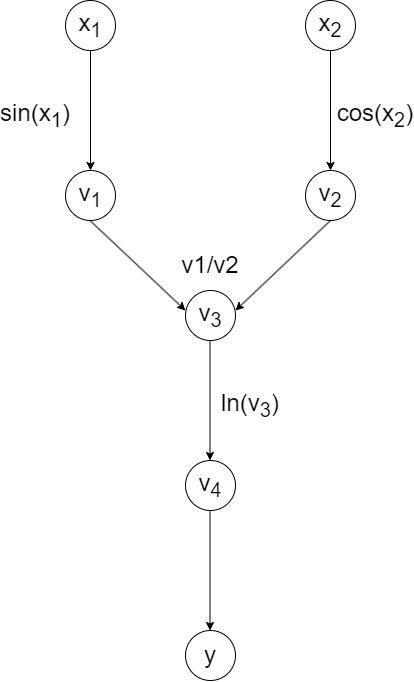
\includegraphics[scale = 0.34]{ExampleCompGraph.png}
        \caption{Example Computational Graph}
    \end{wrapfigure}
    Now that we have declared our intermediate variables, we can see how automatic differentiation splits up the original function into elementary ones.
    This then allows use to easily take derivatives. Firstly, we can draw out the computational graph for this function, using our intermediate variables,
    and this can be seen in Figure 7.
    This graph visualizes the forward pass of the function, and how the intermediate variables compose to form our original function.

    Now, when we want to take the derivative with respect to one of these inputs, we can simply reverse through the graph, taking the gradient of each intermediate
    variable, and using the chain rule to give us our final derivative.

    This process would looks as follows: \begin{align}
        \frac{\partial y}{\partial x_1} = \frac{\partial y}{\partial v_4} \cdot \frac{\partial v_4}{\partial v_3} \cdot \frac{\partial v_3}{\partial v_1} \cdot \frac{\partial v_1}{\partial x_1}
    \end{align}

    If we computed each of these derivatives:
    \begin{align}
        \frac{\partial y}{\partial v_4} &= 1\\
        \frac{\partial v_4}{\partial v_3} &= \frac{1}{v_3}\\
        \frac{\partial v_3}{\partial v_1} &= \frac{1}{v_2}\\
        \frac{\partial v_1}{\partial x_1} &= cos(x_1)
    \end{align}

    And finally, evaluating equation $(8)$, as well as substituting our intermediate variables in terms of $x_1$, to obtain $\frac{\partial y}{\partial x_1}$:
    \begin{align}
        \frac{\partial y}{\partial x_1} &= \frac{cos(x_1)}{v_3 \cdot v_2}\\
        &= \frac{cos(x_1)}{v_1}\\
        &= \frac{cos(x_1)}{sin(x_1)}
    \end{align}

    This process of traversing through the graph backwards is known as reverse accumulation auto differentiation, and in practice each of the gradients would be
    stored numerically at computation, rather than computing a symbolic version of the final derivative and plugging the values in.

    \subsubsubsection{Reinforcement Learning (RL)} \label{RL Existing Analysis}
    Reinforcement learning aims to capitalize on learning through an environment (similar to how infants learn by playing), without a teacher, to improve computer's
    ability at a given task. Simply put, problems in reinforcement learning involve learning how to map certain situations to certain actions to maximize a reward signal.
    The models are not told what actions to take and instead must explore the environment and available actions to learn what yields the most rewards. In some cases, actions
    may not only affect immediate rewards, but also the possibility and/or size of future rewards.

    \begin{wrapfigure}{l}{0.5\linewidth}
        \centering
        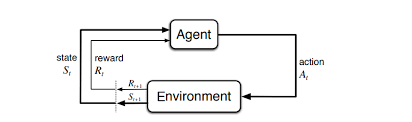
\includegraphics[scale =0.5]{markovprocess.png}
        \caption{Diagram of Markov Decision Process}
    \end{wrapfigure}
    The solution to reinforcement learning problems can be modelled using a markov decision process (A diagram of which can be seen in Figure _). This diagram shows the process of
    one iteration of training. The agent will recieve a state ($S_t$) and then decide on an action to take ($A_t$). This action is sent to the environment, which process the action,
    evaluates the reward gained from that action ($R_t$), and then returns that reward and the next state ($S_{t+1}$).
    
    One challenge that becomes in apparent in reinforcement learning, that is not present in other machine learning methods (supervised and unsupervised), is that of \textit{exploration}
    vs \textit{exploitation}. This problem comes from the fact that to maximize any given reward signal, an agent must take the action which gains the most reward i.e. it must
    \textit{exploit} what it knows, and choose the best action. However, to have knowledge of which action is best at any given state, the agent must have \textit{explored} many different
    actions - in many different states. This challenge will be addressed in more depth later on, during the design of the agent.

    There are two main approaches to reinforcement learning problems, a model-free solution or model solution. Within model-free solutions there is another two categories of policy optimization
    and Q-learning. In policy optimization, the agent learns a policy which maps states to actions. There are two types of these policies - deterministic and stochastic. A deterministic policy
    maps without uncertainty i.e. the agent will take the same action given the same state. Stochastic policies on the other hand output a distribution which maps a state to the probability of 
    each action.

    \begin{wrapfigure}[17]{l}{0.4\linewidth}
        \centering
        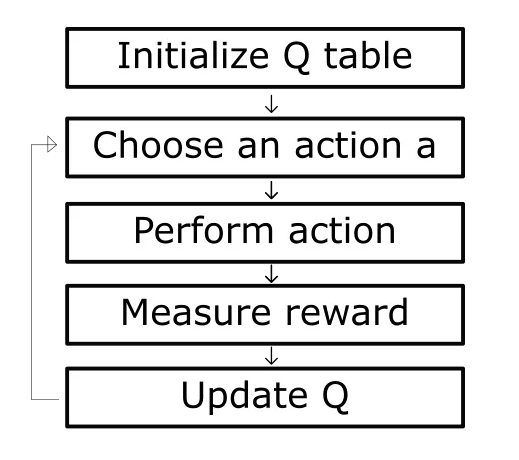
\includegraphics[scale=0.4]{qlearning.PNG}
        \caption{Representation of Q-learning process}
    \end{wrapfigure}
    Q-learning can be represented as a tabular learning method, and works by learning the value of a function - usually $Q(s, a)$ - which represents how successful an action was at
    a certain state. Each of these values is stored in the 'table' and when the model next observes a given state it consolidates the table and chooses the action which was most
    successful in its past experience.

    For model-based solutions, the models 'know' the rules of the games and learn from planning and construct a functional representation of the environment. This is different to non-model
    based which aims to learn by trial-and-error and experience. AlphaZero for example would be defined as a model-based agent. To better define this, if the agent is able to forecast the reward
    of an action given any state, allowing it to plan what actions to take, it is model-based.

    Model-based solutions are best when trying to optimize the reward for a task - such as playing chess. Whereas model-free solutions are best for tasks such as self-driving cars (as a model-based
    approach may run over a pedestrian just to try and complete the journey in the shortest time).

    \subsubsubsection{AlphaZero}
    As mentioned before, AlphaZero is model-based - but how exactly it works is unique and does not have a naming convention like Q-learning.

    AlphaZero uses a process called Monte Carlo Tree Search (MCTS) to build a tree of future variations of a game. This tree is built depth first - so only begins building a new branch, when the state in the
    branch currently being explored is terminal. When building this tree, MCTS must select a child node - if all possible new actions have been exhausted. To do this a formula called the upper confidence 
    bound (UCB) is used. The UCB formula can be seen below.
    \begin{align}
        UCB = \frac{w_i}{n_i} + C\sqrt{\frac{ln(N_i)}{n_i}}
    \end{align}
    
    In this equation, $w_i$ represents the number of wins a node has, $n_i$ represents the number of visits a node has, $N-i$ represents the number of visits the parent node has, and $C$ is a coefficient which
    controls the levels of exploration in the MCTS model.
    Also, after each branch has reached a terminal state the MCTS backpropogates and records how many times each node has been visited, and how many times that node has lead to a winning terminal state. 
    Using this recorded data, the MCTS model can build a distribution which models the probability of winning the game for each action in the current state. This allows the model to 'learn' the rules
    of the game, as illegal actions will have a probability of 0. This distribution can also be called the MCTS' policy.

    To improve this process, AlphaZero uses a neural network to help prune some branches of the tree which can be assumed to lead to a losing state. This allows the MCTS to search only more effective
    lines of play. The exact algorithm for this can be found in \myhy{sec:IDoA}{Identification of Algorithms}
    


    
    \subsubsection{Similar Systems}
    \begin{wrapfigure}[14]{r}{0.5\linewidth}
        \centering
        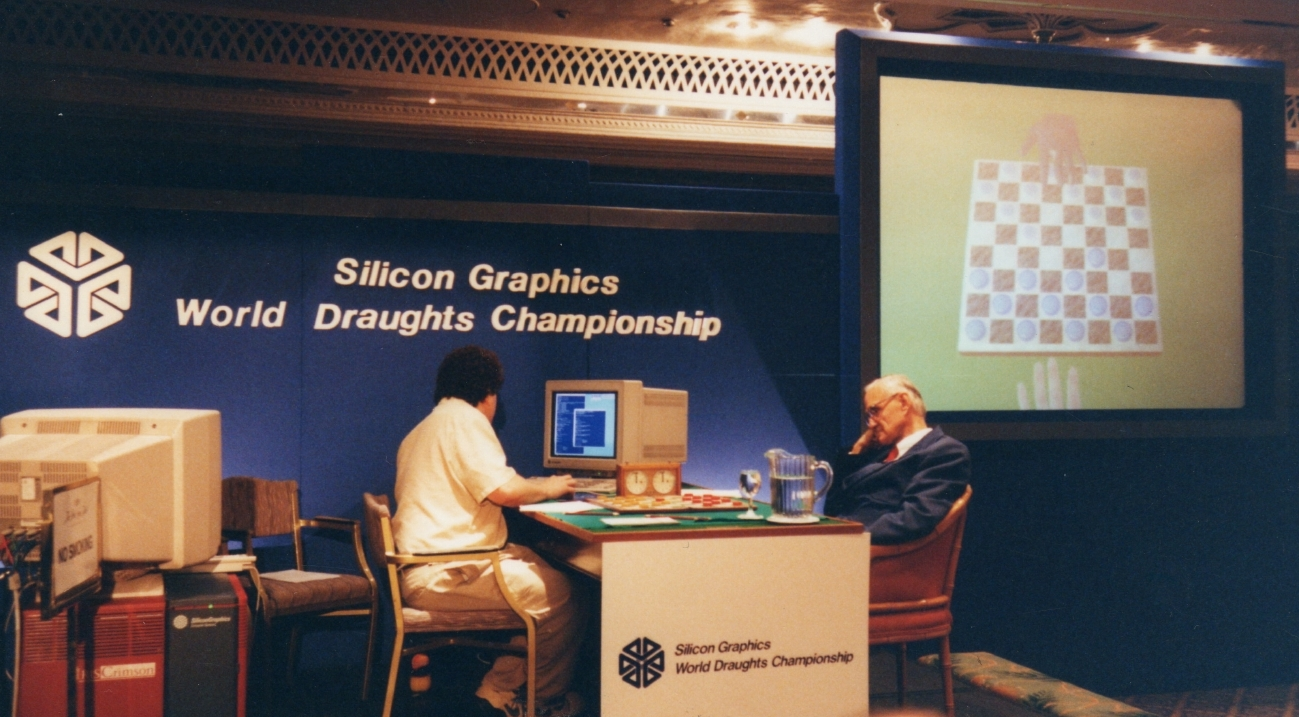
\includegraphics[scale=0.145]{1992Tinsleymatch.jpg}
        \caption{Image of Chinook playing a game of checkers - 1992}
    \end{wrapfigure}
    Chinook is a checkers playing computer program that was developed at the University of Alberta between
    1989 and 2007. The program utilises an opening book, deep-search algorithms alongside a position evaluation function
    and a solved endgame database for positions with 8 pieces or fewer.
    All of Chinook's knowledge has been programmed in by humans, with no use of an artificial intelligence model. Despite this,
    Chinook managed to beat the checkers world champion at the time of 1995, and after this no longer competed, but instead was
    tasked with solving checkers. (A solved game is one where the outcome can be predicted from any position) - and this was achieved in 2007.

    \begin{wrapfigure}[16]{l}{0.5\linewidth}
        \centering
        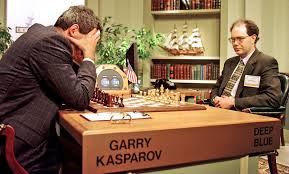
\includegraphics[scale=0.7]{download.jpg}
        \caption{Chess champion Garry Kasparov loses to Chess engine - 1997}
    \end{wrapfigure}
    Other similar systems include chess engines - of which there is a multitude. Chess engines operate similarly to Chinook, creating trees
    of possible moves and using a minimax algorithm, as well as alpha-beta pruning to determine the best move. Additionally, there are some
    chess engines which use reinforcement learning, such as Google DeepMind's AlphaZero engine. This engine has also been trained on games
    such as Go and Shogi. AlphaZero is trained mainly using self-play, where the AI plays against itself and then learns from those games.
    In a 100 game match against StockFish (one of the most popular chess engines) AlphaZero won 28 games, lost 0 and drew the remaining 72.
    This shows the power of reinforcement learning as a tool for board games and its possibility to be used for checkers.

    For automatic differentiation, some of the most popular systems include PyTorch's autograd, as well as autodiff by JAX. PyTorch has a very
    well developed library for deep-learning alongside it's autograd, as well as extensive documentation. Additionally, autograd is more similar
    to regular python than JAX and may be easier to use when first delving into the area. However, JAX builds on top of autograd and accelerates
    the linear algebra using an XLA backend. This backend optimizes operations for CPU's GPU's and TPU's as well as using a just-in-time compiler
    to decrease runtimes.

    \subsubsection{Interview with third party}
    For my interview, I reached out to an external person who works in the AI industry. We discussed where my time would be most well spent,
    some industry standards I should try and implement as well as some expansionary objectives I could try to include to improve my project.

    To start with, with the large amount of work that needs to be done, if time begins to run short there are lots of out-of-the-box frameworks
    to use and implement (such as PyTorch and JAX - mentioned earlier), while still allowing me to finish my project with sufficient difficulty.
    Secondly, the large proportion of my time should be spent researching and understanding the different solutions available which would best
    suit my problem, and how they are implemented. This research should include, but not be restricted to: reinforcement learning solutions for
    other games (such as Go and Chess), different attributes of reinforcement learning models and which environments they are most capable in, as well
    as research on the overheads of similar models.

    It is very important that the correct solution is chosen, so minimal time is spent on implementation.

    As for possible objectives:
    \begin{center}
        \begin{tabular}{|m{15em}|m{15em}|}
            \hline 
            Objective & Reasoning \\
            \hline
            Leverage GPU cores for linear algebra computations & Allows parallelization and will increase computation speeds  \\      
            \hline
            Wrap the console checkers board in a GUI & Much easier for users to use and understand \\
            \hline
            Use a container such as Docker to produce logs & Much better retracing and debugging capabilities \\
            \hline
            Evaluate the model against Chinook and human players & Allows for rating of model \\
            \hline
        \end{tabular}
    \end{center}

    
    \subsection{Modelling of the problem}

    \subsubsection{Identification of Objects}

    \subsubsubsection{Checkers}
    For checkers, we will need two classes, a checkers board/environment and a checkers game. The environment will be used for training the agent and It will require methods that
    execute an action in the environment, as well as functions to compute the available moves and check for a win. An example of UML for this environment can be seen below. 

    \begin{figure}[h]
        \centering
        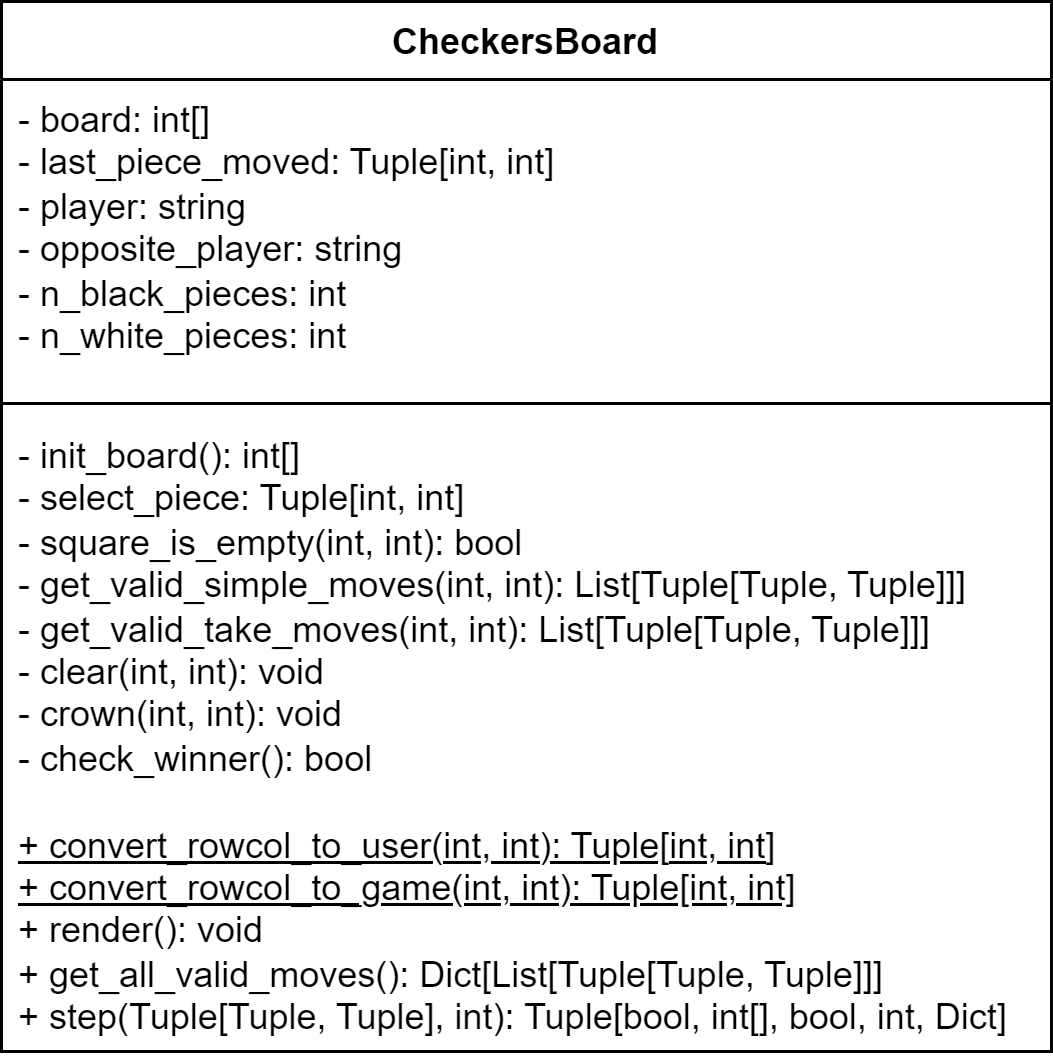
\includegraphics[scale = 0.24]{DraughtsUMLdrawio.png}
        \caption{UML for checkers/checkers game}
    \end{figure}

    The checkers game varies only slightly and will inherit from the checkers board. It will however add some functionality such as a GUI and the ability to choose different
    models to play against (such as just the MCTS or the full agent). Additionally, it should allow two people to play each other as checkers usually would.

    \subsubsubsection{Automatic Differentiation Engine}
    \begin{wrapfigure}{l}{0.5\linewidth}
        \centering
        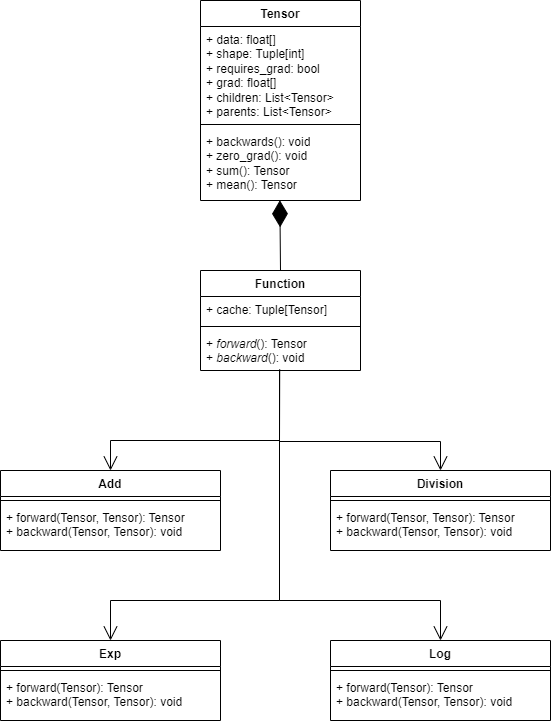
\includegraphics[scale=0.02]{AutoDiffUML.drawio.png}
        \caption{Example UML for Auto Diff}
    \end{wrapfigure}
    The automatic differentiation engine will be based off of the 'Tensor' object. This object will be similar to a matrix but have some additonal
    attributes, such as its gradient and if its gradient requires computing. If the tensor does require a gradient then it will also store its parent
    tensors, which will be used for the backward DFS of the computational graph.

    Additionally, all operators for the tensor object will have to be overridden to allow for gradient computation if the tensor requires it.
    The tensor class will also have functions to zero out the gradient as well as begin the backwards traversal through the computational graph. Below is an example
    of some possible UML for the automatic differentiation library.

    Tensor operations will all have a backward and forward method - inherited from the function class. These functions will represent elementary functions (Addition, Division, Log, etc.). 
    The operations such as sum and mean, that operate on the tensor itself will also be represented by a function object.

    \subsubsubsection{Neural Network Library}
    Their will be a large collection of objects inside of the neural network library, all based around the functionality provided by the tensor object.
    Firstly, the parameter class will allow for tensors of a given shape to be created and act as parameters for a network - this will also help with backpropogation.
    The module object will have a parameters property which yields every parameter related to that module. This module class is what all layers will inherit from. It will also
    have methods to zero out the gradients of all parameters.

    Secondly, their will be classes for each different type of layer (dense and activations). The dense layer will have attributes which store the parameters required
    for computation as well as a method to complete the forward pass through the layer. Activation functions will compute the forward pass, as well as store the gradient function
    for any tensors which require it. The activation layers will not need any attributes as the have no parameters.

    The optimizer class is the base class for any optimizers such as stochastic gradient descent or momentum-based gradient descent. This class will have attributes which store
    the learning rate as well as any parameters the optimizer is related to. It will also have virtual methods - which will be overriden by the specific optimizer classes - of
    a step (which updates all parameters), a function to zero the gradient of all parameters and finally a function to add parameters.

    Below is an inheritance diagram for the Neural Network Library, without any attributes and methods.

    \begin{figure}[h]
        \centering
        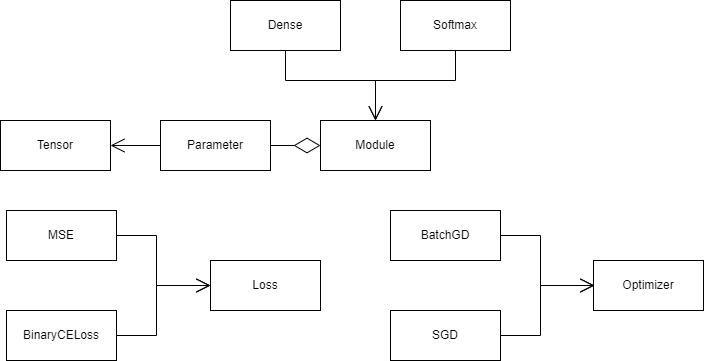
\includegraphics[scale=0.5]{NNUML (simple).drawio.png}
        \caption{Inheritance diagram for Neural Network Library}
    \end{figure}


    \pagebreak
    \subsubsubsection{Reinforcement Learning Solution}
    The final solution will also require a large set of classes including: a network class - to output the model policy and predicted value; a monte carlo tree searach (MCTS) class to compute
    a search of available actions to train the network towards - composed of a node class to make up this tree - and finally an agent class which abstracts the processes of the previous classes. \\

    \begin{figure}[h]
        \centering
        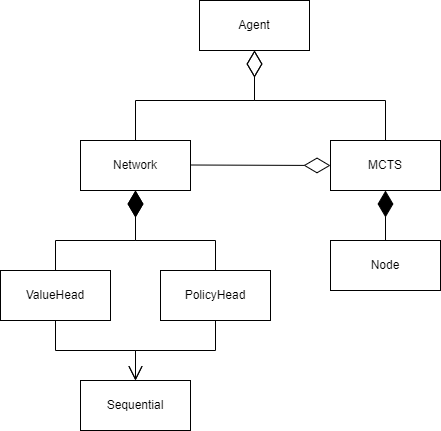
\includegraphics[scale=0.5]{RLSolutionUML.png}
        \caption{Reinforcement Learning Solution UML}
    \end{figure}
    


    \pagebreak
    \subsubsection{Identification of algorithms} \label{Analysis-IoA}
    \label{sec:IDoA}
    \subsubsubsection{Automatic Differentiation Engine}
    The auto-diff engine will use a recursive DFS of the computational graph to calculate gradients. It uses a DFS as any of the computational graphs that built are directed acyclical graphs,
    and therefore DFS provides a way to search the whole graph in O(n) time. Some pseudocode for this search can be seen below.

    \begin{algorithm} 
        \caption{Backward Function of Tensor}\label{alg:cap}
        \begin{algorithmic}
        \Function{Backward}{Tensor self, Array grad, Tensor out}
        \Ensure t.requiresGrad is True \Comment{t is the tensor being called to start DFS}
        \If{t.Grad is None}
            \State grad $\gets \begin{bmatrix}
                1 & 1 & 1 & \hdots
            \end{bmatrix}$ in shape of t.data
        \EndIf
        
        \State t.Grad += grad

        \If{t.Operation is not None}
            \State t.Operation.backward(t.Grad, t)
        \EndIf

        \EndFunction
        \end{algorithmic}
    \end{algorithm}

    \begin{algorithm}
        \caption{General Backward Function of a Tensor Operation}\label{alg:cap}
        \begin{algorithmic}
        \Function{backward}{Operation self, Array grad, Tensor t}
        \State savedTensors $\gets$ self.cache.0
        
        \For{tensor in savedTensors}
        \If{tensor.requiresGrad is True}
        \State newGrad $\gets \frac{\partial output}{\partial tensor}$ \Comment{Computed by chain rule, specific for each operation}
        \If{broadcastedDims}
        \State Remove broadcasted dims from newGrad \Comment{newGrad.shape should equal tensor.shape}
        \EndIf
        \State tensor.backward(newGrad, t)
        \EndIf
        \EndFor
        \EndFunction
        \end{algorithmic}
    \end{algorithm}

    \subsubsubsection{Neural Network Library} \label{Analysis-IofA-NNLib}
    The two main algorithms in the neural network library are the forward pass and the backward pass through a collection of layers. Pseudocode for these can also been seen below.
    \begin{algorithm}
        \caption{Forward pass through collection of layers}\label{alg:cap}
        \begin{algorithmic}
        \Function{forward}{Module model, Tensor input}
        \State output $\gets$ input
        
        \For{layer in model.layers}
        \State output $\gets$ layer.forward(output) \Comment{layer's forward function depends on layer type (Dense/Conv)}
        \EndFor
        return output
        \EndFunction
        \end{algorithmic}
    \end{algorithm}

    \begin{algorithm}
        \caption{Training process of a module}\label{alg:cap}
        \begin{algorithmic}
        \Function{fit}{Module model, Optimizer optim, Loss l, Tensor x, Tensor y, int epochs = 100, int verbose = 1}
        \State startTime $\gets$ time.now()
        
        \For{epoch in epochs}
        \State prediction $\gets$ model.predict(x) \Comment{Get predictions}
        \State loss $\gets$ l(y, prediction) \Comment{Calculate how far predictions are from true}
        \State optimizer.zero_grads() \Comment{Reset gradients of parameters}
        \State loss.backwards() \Comment{Calculate gradients of loss}
        \State optimizer.step() \Comment{Update parameter values using calculated gradients}

        \If{verbose is 1}
        \State print(epoch, loss)
        \EndIf

        \EndFor
        print(time.now() - startTime) \Comment{Total time elapsed}
        \EndFunction
        \end{algorithmic}
    \end{algorithm}
    
    \pagebreak
    \subsubsubsection{Reinforcement Learning Solution}
    For the reinforcement learning, one of the most important algorithms is the MCTS which is similar to a DFS. This takes all
    the available moves in the checkers environment, selects one at random and continues this process until a terminal state is reached.
    After the terminal state is reached, reward values (+1 for win, -1 for loss, 0 for draw) are backrpopagated through the nodes.
    If all possible available moves have been exhausted at a given node then it selects one using an upper confidence bound (UCB) formula.
    The general algorithm can be seen in pseudocode below (as well as the nodes expand function).

    \begin{algorithm}
        \caption{MCTS Tree Building Function}\label{alg:cap}
        \begin{algorithmic}
        \Function{buildTree}{currentBoardState}
        
        \State self.root $\gets$ currentBoardState

        \For{seach in numberOfSearches}
        \State node $\gets$ self.root \Comment{Return to start of tree for each search}
        \If{node.brancesAvailableToExpand == 0}
        \State node $\gets$ node.select_child()
        \EndIf
        
        \While{node.terminal is False AND node.branchesAvailableToExpand $>$ 0}
        \State node $\gets$ node.expand() \Comment{Depth-first expansion until terminal state}
        \EndWhile

        \State node.backpropogate(node.reward)
        \EndFor
        \EndFunction
        \end{algorithmic}
    \end{algorithm}
    
    The second algorithm is the process of the final agent model selecting its actions and can be seen on the next page.

    \begin{algorithm}
        \caption{Agent Policy Selection}\label{alg:cap}
        \begin{algorithmic}
        \Function{trainAgent}{self, initialNeuralNetwork, hyperParameters}
        
        \State nnPrevious $\gets$ initialNeuralNetwork
        \For{mctsEpoch in hyperParameters.mctsEpochs}
            \State trainingExamplesList $\gets$ SPV(hyperParameters.maxExamples)
            \For{episode in hyperParameters.episodes}
                \State examples $\gets$ list()
                \State game $\gets$ new CheckersGame
                \While{!game.terminated}
                    \State mcts $\gets$ MCTS(nnPrevious, game.currentBoardState, hyperParameters).buildTree()
                    \If{game.step $<$ hyperParameters.Threshold}
                        \State action $\sim$ mctsPolicy.getPolicy() \Comment{Select random move}
                    \Else
                        \State action $\gets$ mcts.getAction()
                    \EndIf
                    \State examples.append((game.currentBoardState, mcts.getPolicy(), initialNeuralNetwork.value))
                \EndWhile
                \State trainingExamplesList.append(examples)
                \For{networkEpoch in hyperParameters.networkEpochs}
                    \State batch $\gets$ trainingExamplesList.getBatch(hyperParameters.batchSize)
                    \State nnNew $\gets$ nnPrevious.train(batch, hyperParameters)
                \EndFor
                \State numberNNNewWins = 0
                \For{compareGame in hyperParameters.compareGames}
                    \State game $\gets$ new CheckersGame
                    \While{!game.terminated}
                        \If{game.player == player1}
                            \State action $\gets$ MCTS(nnPrev, game.currentBoardState, hyperParameters).getAction()
                        \ElsIf{game.player == player2}
                            \State action $\gets$ MCTS(nnNew, game.currentBoardState, hyperParameters)
                        \EndIf
                    \EndWhile
                \EndFor
                \State nnNewWinPct = numberNNNewWins/hyperParameters.compareGames
                \If{nnNewWinPct $>$ hyperParameters.replaceThresholdPct}
                    \State nnPrev $\gets$ nnNew
                \EndIf
            \EndFor
        \EndFor
        \State \Return nnPrev
        \EndFunction
        \end{algorithmic}
    \end{algorithm}

    
    \pagebreak
    \subsubsection{Mathematical Formulae} \label{Analysis-MathematicalFormulae}
    \subsubsubsection{Automatic Differentiation Engine}
    In this section I will simply define the formulas for the forward and backward pass of many different functions that will be implemented
    into the autograd library.
    \subsubsubsubsection{Addition}
    \subsubsubsubsubsection{Forward}
    \begin{align}a + b = y\end{align}
    \subsubsubsubsubsection{Backward}
    \begin{align}\frac{\partial y}{\partial a} = 1 + 0\end{align}\\
    \begin{align}\frac{\partial y}{\partial b} = 0 + 1\end{align}

    \subsubsubsubsection{Negation}
    \subsubsubsubsubsection{Forward}
    \begin{align}y = -a\end{align}
    \subsubsubsubsubsection{Backward}
    \begin{align}\frac{\partial y}{\partial a} = -1\end{align}

    \subsubsubsubsection{Multiplication}
    \subsubsubsubsubsection{Forward}
    \begin{align}a \cdot b = y\end{align}
    \subsubsubsubsubsection{Backward}
    \begin{align}\frac{\partial y}{\partial a} = b\end{align}
    \begin{align}\frac{\partial y}{\partial b} = a\end{align}

    \subsubsubsubsection{Division}
    \subsubsubsubsubsection{Forward}
    \begin{align}\frac{a}{b} = y\end{align}
    \subsubsubsubsubsection{Backward}
    \begin{align}\frac{\partial y}{\partial a} = \frac{1}{b}\end{align}
    \begin{align}\frac{\partial y}{\partial b} = -\frac{a}{b^2}\end{align}

    \subsubsubsubsection{Matrix multiplication}
    \subsubsubsubsubsection{Forward}
    \begin{align}
        AB = Y &&\text{where A and B are matrices}
    \end{align}
    \subsubsubsubsubsection{Backward}
    \begin{align}\frac{\partial Y}{\partial A} = B^T\end{align}
    \begin{align}\frac{\partial Y}{\partial B} = A^T\end{align}

    \subsubsubsubsection{Powers}
    \subsubsubsubsubsection{Forward}
    \begin{align}a^b = y\end{align}
    \subsubsubsubsubsection{Backward}
    \begin{align}\frac{\partial y}{\partial a} = ba^{b-1}\end{align}
    \begin{align}\frac{\partial y}{\partial b} = a^bln(a)\end{align}

    \subsubsubsubsection{Mean}
    \subsubsubsubsubsection{Forward}
    \begin{align}\frac{\sum A}{n} = y, && A = (x_0, x_1, x_2, \hdots x_n) \end{align}
    \subsubsubsubsubsection{Backward}
    \begin{align} \frac{\partial y}{\partial A} = B, && B = ({\frac{1}{n}}_0, {\frac{1}{n}}_1, {\frac{1}{n}}_2 \hdots, {\frac{1}{n}}_n) \end{align}
    
    \subsubsubsubsection{Sum}
    \subsubsubsubsubsection{Forward}
    \begin{align} \sum A = y, && A = (x_0, x_1, x_2, \hdots x_n) \end{align}
    \subsubsubsubsubsection{Backward}
    \begin{align} \frac{\partial y}{\partial A} = B, && B = ({1}_0, {1}_1, {1}_2 \hdots, {1}_n) \end{align}

    \subsubsubsubsection{Natural Log}
    \subsubsubsubsubsection{Forward}
    \begin{align} ln(a) = y \end{align}
    \subsubsubsubsubsection{Backward}
    \begin{align} \frac{\partial y}{\partial a} = \frac{1}{a} \end{align}

    \subsubsubsubsection{Exponentation}
    \subsubsubsubsubsection{Forward}
    \begin{align} e^a = y \end{align}
    \subsubsubsubsubsection{Backward}
    \begin{align} \frac{\partial y}{\partial a} = e^a \end{align}

    \subsubsubsubsection{Conv2D}
    \subsubsubsubsubsection{Forward}
    \begin{align} Y_i = B_i + \sum_{j=1}^{n}X_j \star K_{ij}, \hspace{1cm} i = 1 \dots d\end{align}
    Similar to the current systems, the star denotes the valid cross-correlation of the two matrices.\\
    \textbf{Example of cross-correlation}\\
    Cross correlation can be imagined as placing the kernel ontop of the input and summing the products of the elemts which overlap, and then moving the kernel and repeating the process.
    \begin{align}
        \begin{bmatrix}
            1 & 6 & 2 \\
            5 & 3 & 1 \\
            7 & 0 & 4 \\
        \end{bmatrix} \star \begin{bmatrix}
            1 & 2 \\
            -1 & 0 \\
        \end{bmatrix} &= \begin{bmatrix}
            1 \cdot 1 + 2 \cdot 6 + -1 \cdot 5 + 0 \cdot 3 & 1 \cdot 6 + 2 \cdot 2 + -1 \cdot 3 + 0 \cdot 1 \\
            1 \cdot 5 + 2 \cdot 3 + -1 \cdot 7 + 0 \cdot 0 & 1 \cdot 3 + 2 \cdot 1 + -1 \cdot 0 + 0 \cdot 4
        \end{bmatrix}\\
        &= \begin{bmatrix}
            8 & 7 \\
            4 & 5
        \end{bmatrix}
    \end{align}

    This method of cross-correlation is known as valid cross correlation (where the upper left element of the kernel 
    begins on the upper left element of the input).
    \subsubsubsubsubsection{Backward}
    
    In this backward function, $\frac{\partial Z}{\partial Y}$ will denote the gradient being recieved from upstream.
    \begin{align}
        \frac{\partial Z}{\partial B_i} &= \frac{\partial Z}{\partial Y_i}\\
        \frac{\partial Z}{\partial K_{ij}} &= X_j \star \frac{\partial Z}{\partial Y_i}\\
        \frac{\partial Z}{\partial X_i} &= \sum_{i=1}^{d}\frac{\partial Z}{\partial Y_i} * K_{ij}
    \end{align}

    The asterisk in the final expression represents the full convolution operation, which is the same as a full cross-correlation, but
    with the kernel rotated 180 degrees. Additionally, a full correlation begins the operation with the bottom left elemnt of the kernel
    being placed upon the top left element of the input - and then the sliding and summing of products process remains the same.
    
    \subsubsubsection{Neural Network Library}
    \subsubsubsubsection{Activation Layers}
    In both dense and convolutional layers, the only operation that is occuring is multiplication and/or matrix multiplication. Graphically,
    these operations only create linear transformations however in machine learning some problems require non-linearity. To allow for non-linearity
    neural networks use activation layers which are non-linear functions, normally places between layers.
    
    \subsubsubsubsubsection{Tanh}
    \begin{align}
        tanh(x) = \frac{e^x - e^{-x}}{e^x + e^{-x}}
    \end{align}

    \subsubsubsubsubsection{Sigmoid}
    \begin{align}
        S(x) = \frac{1}{1 + e^{-x}}
    \end{align}

    \subsubsubsubsubsection{Softmax}
    The softmax function is used to turn a vector into a probability distribution. For example, if we had data in the shape (batches, classes) and we wanted to getAction
    the probability of each batch being in a certain class we would use the softmax function across the axis with the number of class, in this case axis 1.
    \begin{align}
        \sigma(x) = \frac{e^x}{\sum e^x} \hspace{10mm} \text{Sum across axis with number of classifications in x}
    \end{align}

    \subsubsubsection{Reinforcement Learning Solution}
    \subsubsubsubsection{UCB Formula}
    The UCB formula is used in MCTS to select the most favourable child when the parent node has been fully expanded. The formula can be seen below, where
    $N_i$ is the number of visits the parent node has, $n_i$ is the number of visits the child node has and $w_i$ is the value count that the node holds. The
    value count is updated each iteration during backpropogation. Finally, $C$ is a coefficient which determines the levels of exploration and exploitation.

    \begin{align}
        UCB(Node_i) = \frac{w_i}{n_i} + C \sqrt{\frac{ln N_i}{n_i}}
    \end{align}

    \subsection{Set of objectives}
    \subsubsection{Checkers Game}
    \begin{enumerate}
        \item An easy-to-use and intuitive graphical interface for the checkers game
        \begin{enumerate}
            \item A working version of checkers - obeying all rules stated in \myhy{checkers}{1.2.1.1}
            \item A small text tutorial on the rules of checkers
            \item A visual representation of the checkers board
            \item A method of displaying all legal available moves in a selected position
            \item Informative error messages if an illegal move is attempted
        \end{enumerate}
        \item Implementation of various decision-making agents for users to play against
        \begin{enumerate}
            \item Option for the user to choose which agent to play against (MCTS, Full Agent)
            \item Ability to adjust hyperparameters of the agents from the checkers game interface (see \myhy{RLS Objs}{RLS Objectives a-e})
            \item Information printed to the user pertaining to the agent's decision-making progress
        \end{enumerate}
    \end{enumerate}
    \subsubsection{Autodifferentiation engine}
    \begin{enumerate}
        \item A unit-tested autograd engine capable of calculating derivatives on a variety of functions inlcuding:
        \begin{enumerate}
            \item Addition
            \item Negation
            \item Multiplication
            \item Division
            \item Matrix Multiplication
            \item Powers
            \item Mean
            \item Sum
            \item Natural Log
            \item Exponentiation
            \item Transpose
            \item Padding
            \item 2D Convolution
        \end{enumerate}
    \end{enumerate}
    \subsubsection{Neural Network Library} 
    \begin{enumerate} 
        \item A modular machine learning library including:
        \begin{enumerate}
            \item The ability to save a model
            \item Support for storing a collection of layers/modules
            \item Dense/Fully Connected Layer
            \item 2D Convolution Layer
            \item Reshape Layer
            \item Activation Layers:
            \begin{enumerate}
                \item ReLU
                \item Softmax
                \item Sigmoid
                \item Tanh
            \end{enumerate} 
            \item Gradient descent optimization
            \item Loss Functions:
            \begin{enumerate}
                \item Mean Squared error
                \item Binary Cross Entropy Loss
                \item AlphaZero's Loss Function
            \end{enumerate}
        \end{enumerate}
    \end{enumerate}

    \subsubsection{Reinforcement Learning Solution} \label{RLS Objs}
    \begin{enumerate}
        \item A training algorithm with hyperparameters of:
        \begin{enumerate}
            \item Number of example games to be played
            \item Number of comparison games to be played
            \item Number of searches the MCTS completes
            \item The exploration exploitation coefficient for UCB in MCTS
            \item The percentage of comparison games the new network must win to replace the previous
            \item The number of epochs for neural network training
            \item The number of iterations where a new network is trained
        \end{enumerate}
        \item The functionality to load a saved agent and play against it
    \end{enumerate}

    \section{Design}

    \subsection{File Structure and Project Organisation} \label{File-Structure}
    \dirtree{%
        .1 *ns-*eec-*te-*cg-*rt.
        .1 poetry.lock.
        .1 pyproject.toml.
    }
    At the very top level of my file structure I have a poetry.lock and a pyproject.toml file. These files are automatically generated by
    a python package called poetry. This package provides exceptionally easy dependency and virtual environment management. Allowing me to
    setup machines other than my own - to train the model - more easily. 
    The final file inside of this directory actually represents a collection of files - with each * denoting a different value that each of the 
    parameters for the final model can take (with the two letters allowing me to identify said parameter). These files are created using python's built in pickle object serialization library.
    \dirtree{%
        .1 nea-code.
        .2 AlphaMCTSSelfPlay.py.
        .2 AlphaModel.py.
        .2 CheckersGamePvP.py.
        .2 CheckersGuiGame.py.
        .2 MCTSSelfPlay.py.
        .2 PvMCTS.py.
        .2 TestNNXOR.py.
        .2 TrainAgent.py.
    }
    At one level inside of my main code-storing file I have files that run main operations in my code. This includes specific game loops, such as getting the user to play 
    vs MCTS - as well as processes such as beginning agent training and testing of the Neural Network Library using a simple problem such as XOR.
    \dirtree{%
        .1 nea-code.
        .2 agent.
        .3 agent.py.
        .3 consts.py.
        .3 memory_types.py.
        .3 __init__.py.
    }
    Inside of nea-code I also create a subdirectory for each module of my project. In the above example this modeule is the agent class. As well as storing the file which defines the agent class (agent.py)
    it also contains an \_\_init\_\_.py file (which allows python to recognise the subdirectory of nea-code as a module and defines what dependencies to import when this module is called), a consts.py (which contains
    values, and functions to create values, which do not change throughout the running of the code) and a memory_types.py file, where dataclasses such as SAP and SPV (which will be defined later on. hereTODO ADD LINK) are defined.
    \dirtree{%
        .1 nea-code.
        .2 checkers_gui.
        .3 buttons.py.
        .3 checkers_gui.py.
        .3 consts.py.
        .3 helpers.py.
        .3 __init__.py.
        .4 media.
        .5 images.
        .6 black_k.png.
        .6 black_r.png.
        .6 checkers_board_no_pieces.png.
        .6 white_k.png.
        .6 white_r.png.
    }
    The next module is the GUI add-on for the checkers game. Similarly to the agent module, it contains \_\_init\_\_.py, consts.py, a main class definition file (checkers\_gui.py) and other class definitions file (buttons.py). 
    However, the checkers GUI module also contains a helpers.py file - which holds onto functions that are helpful relevant to the module as well as a subtree of media/images/ which contains the .png's of the different sprites used in the GUI.
    \dirtree{%
        .1 nea-code.
        .2 console_checkers.
        .3 checkers_game.py.
        .3 consts.py.
        .3 jit_functions.py.
        .3 utils.py.
        .3 __init__.py.
    }
    Inside of the next module (console\_checkers) we have again an init, consts and main defintion file. On the other hand, instead of a helpers.py file there is a utils.py. The difference here is that
    utils.py contains utility functions not strictly relevant to the module. For example, this utils.py contains a funtion which clears the console (a process which would not be limited to the console\_checkers module).
    Another difference is the presence of the jit_functions.py file. Inside of this module there are lots of functions which run only using primitive types, and have a polynomial time complexity. To reduce the impact this 
    has on performance I use a python package called numba, which contains a just-in-time compiler (jit) to speed up these functions.
    \dirtree{%
        .1 nea-code.
        .2 mcts.
        .3 consts.py.
        .3 mcts.py.
        .3 __init__.py.
    }
    This MCTS module contains definitions of the MCTS classes, again with a consts and init file.
    \dirtree{%
        .1 nea-code.
        .2 ml.
        .3 __init__.py.
        .3 autograd.
        .4 consts.py.
        .4 convolve_funcs.py.
        .4 jit_functions.py.
        .4 tensor.py.
        .4 test_autograd.py.
        .4 helpers.py.
        .4 __init__.py.
        .3 nn.
        .4 layers.py.
        .4 optimizers.py.
        .4 __init__.py.
    }
    In the above snippet I have defined a module named ml (for machine learning), which contains two submodules of autograd and nn - which contain the autodifferentiation engine and neural
    network library respectively. The nn submodule has a similar contents as the modules talked about previously, with layers.py defining the main classes, and optimizers.py then defining classes
    of optimizers to be used alongside the defined layers. The autograd submodule however has a few differences. It also has a jit_functions and helpers file but additionally contains a convolve_funcs.py and
    test_autograd.py file. These files are unique to the autograd module. The convolve_funcs has definitions for complex matrix operations such as convvolution and cross-correlation, and the test_autograd file
    contains unit tests (run using pytest) to evaluate and ensure the accuracy of the autodifferentiation engine.
    \dirtree{%
        .1 nea-code.
        .2 network.
        .3 network.py.
        .3 __init__.py.
    }
    The final module is network, which contains the definitions for compositions of different layers from the nn module - which then build to form the model that is contained within the reinforcement
    learning agent.
    \subsection{Checkers}
    The checkers game solution will be split into a console based version (that will be the main way for the agent to interact with the game) and
    an additonal class built ontop of this console solution which provides a GUI.

    \subsubsection{Data Structures}
    When defining data structures such as tuples, a comma followed by an ellipses indicates another item which is of the same type as most recently defined item
    in the tuple. e.g. tuple[int,...] = tuple[int, int]
    \subsubsubsection{Console Solution}
    \begin{center}
        \begin{tabular}{|m{10em} | m{12em} | m{15em}|}
            \hline 
                Item & Data Structure & Reasoning and Usage \\
            \hline
            \hline
                Board & 2D Array & Easy and logical to index into specific squares as well as render. \\
            \hline
                Last Moved Piece & tuple[int,...] & Represents position of the piece most recently moved - easy to reaccess.\\
            \hline
                Action & tuple[tuple[int,...],...] & First tuple inside of the outer tuple represents the piece being moved, and the second
                inside tuple represents where it is being moved to which allows for easy indexing into the board array.\\
            \hline
        \end{tabular}
    \end{center}
    For a single game of checkers, an upper bound for the number of unique states that can be presented on the board can be calculated as follows (this is useful for getting a gauge
    of the size of training sets compared to the possible set of states):\\

    \noindent Let $0 <= w <= 12$ and $0 <= b <= 12$  where $w,b \in \mathbb{Z}$\\
    Then,
    \begin{align}
        {32}\choose{w}
    \end{align}
    Is the number of ways to play $w$ white pieces on the board, and
    \begin{align}
        {32-w}\choose{b}
    \end{align}
    Is the number of ways to play $b$ black pieces, given $w$ white pieces already occupy a square.
    And for each piece, it can be a king or a regular piece, so we multiply by a factor of $2^{w+b}$.
    Finally to find the number of legal configurations for all $w$ and $b$:
    \begin{align}
        \sum_{b=0}^{12}\sum_{w=0}^{12} {{32}\choose{w}} {{32-w}\choose{b}} 2^{w+b} \approx 2.3\times10^{21}
    \end{align}
    Note: Not all of these positions can be reached via a sequence of legal moves - and the actual number (from
    the paper "Checkers is solved") is $\approx 5 \times 10^{20}$

    Additonally, the set of all possible actions can be written as follows:
    \begin{align}
        R &= \{0,1, ... ,7\}\\
        C &= \{A, B ..., H\}\\
        \text{Possible Actions} &= \{((x,y), (w,z)) \mid x, w \in R \text{^} y,z \in C\}
    \end{align}

    \subsubsubsection{GUI Add-on}
    \begin{center}
        \begin{tabular}{|m{10em} | m{12em} | m{15em}|}
            \hline 
                Item & Data Structure & Reasoning and Usage \\
            \hline
            \hline
                CheckersGUI & Class & Inherits from console solution and stores information about the game such as the piece the user has selected. \\
            \hline
                Selected Piece & tuple[int,...] & Represents position of the selected piece - easy to index into board array. \\
            \hline
                Main Menu & Class & Stores, displays and allows user to change information regarding the parameters and game mode that the user would like to play with. Also initiates game loops.\\
            \hline
                Button & Class & Provides a simpler to use and understand interface between pygame surfaces and user interactions. \\
            \hline
                Constants & Class[T] & Stored in classes named relevant to the constant. These classes contain constant attributes of whatever type that constant is defined as (e.g to get the rgb code for red would require COLOURS.RED and would return (255, 0, 0)) \\
            \hline
        \end{tabular}
    \end{center}

    \subsubsection{Algorithms}
    The key algorithms for the checkers game are ones which scan the board for all possible moves (divided into two processes, for simple moves and take moves) and the step algorithm which processes an input action for a given board state.
    Below is pseudocode for the take moves and step functions can be found below.

    \begin{algorithm}
        \caption{Get Take Moves}
        \begin{algorithmic}
            \Function{getValidTakeMoves}{CheckersGame self}
                \State moves $\gets$ []
                \For {row in range(BOARD\_SIZE)}
                    \For {col in range(BOARD\_SIZE)}
                        \State piece $\gets$ self.board[row, col]
                        \If {piece is of self.currentColour}
                            \For {direction in self.piecesLegalDirections(piece)}
                                \If {self.inBounds(row + 2*direction[row]) and self.inBounds(col + 2*direction[col])}
                                    \State takingSquare $\gets$ (row + direction[row], col + direction[col])
                                    \State moveToSquare $\gets$ (row + 2 * direction[row], col + 2 * direction[col])
                                    \If {self.board[moveToSquare] = 0 and self.board[takingSquare] = opponentsPiece}
                                        \State moves.append(((row, col), moveToSquare))
                                    \EndIf
                                \EndIf
                            \EndFor
                        \EndIf
                    \EndFor
                \EndFor
                \State \Return moves
            \EndFunction
        \end{algorithmic}
    \end{algorithm}
    The above algorithm is for getting valid take moves. The differences between this algorithm and one that gets
    valid simple moves is that this multiplies all directions by 2 (representing a move over one square and landing on
    the square beyond that). For getting simple moves, these directions will not be multplied. Additionally for getting simple moves,
    the takingSquare variable is not needed - and therefore the check inside the final if statement verifying that the taking square is
    an opponents piece would also not be needed.

    \pagebreak
    \vspace*{17.5mm}
    The step algorithm is key to the console checkers solution. It provides a way for the reinforcement learning model to interact by submitting its actions - 
    having them processed with the next state and the reward for the submitted action returned. This process is exactly as defined in the \myhy{analysis section}{RL Existing Analysis}, a markov decision process.
    In the psuedocode, the return statements have been simplified, but in practice the function would most likely return a tuple containing, at minimum: the next state as a 2D array;
    whether the game is over or not as a bool; the reward for the submitted action in that state ($r, r \in \mathbb{Z} \cap [-1, 1]$)
    \vspace{5mm}

    \begin{algorithm} 
        \caption{Checkers Game Step}
        \begin{algorithmic}
        \Function{Step}{CheckersGame self, ACTION action}
        \If{self.lastPieceMoved is None}
            \State allMoves $\gets$ self.getAllMoves()
            \If{len(allMoves) = 0}
                \State \Return gameOver, loss
            \EndIf
            \If{action not in allMoves}
                \State \Return invalidMove
            \Else
                \State self.movePiece()
            \EndIf
        \ElsIf {self.lastPieceMoved is not None}
            \State allMoves $\gets$ self.getTakeMoves()
            \If {action not in allMoves}
                \State \Return invalidMove
            \Else
                \State self.movePiece()
            \EndIf
        \EndIf

        \If {self.isTakeMove(action)}
            \If {self.doubleMoveAvailable()}
                \State lastMovedPiece $\gets$ action[pieceMoved]
            \EndIf
        \EndIf

        \State self.crownPieces()
        
        \If {self.movesWithoutCapture = 40}
            \State \Return draw
        \ElsIf {self.numberBlackPieces = 1 and self.numberWhitePieces == 1}
            \State \Return draw
        \ElsIf {self.numberOppositePlayerPieces = 0}
            \State \Return win
        \ElsIf {self.movesAvailableForOpponent is False}
            \State \Return win
        \Else
            \State \Return nextState
        \EndIf

        \EndFunction
        \end{algorithmic}
    \end{algorithm}

    \pagebreak
    \subsubsection{User Interface}

    \subsubsubsection{Prototyping} \label{Design-UI-Prototyping}
    \begin{figure}[h]
        \centering
        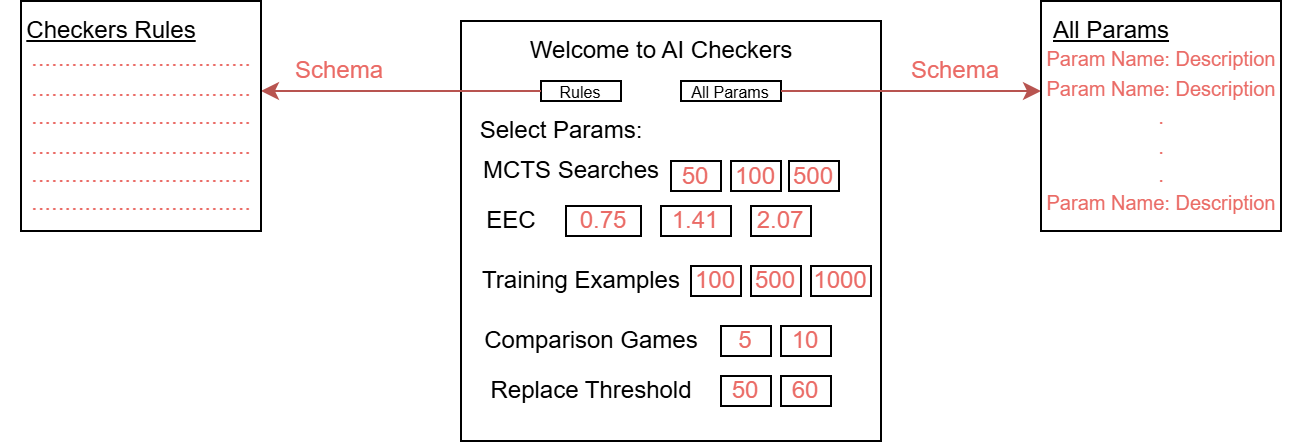
\includegraphics[scale=0.35]{MainMenuPrototype.drawio.png}
        \caption{Prototype Main Menu Design}
    \end{figure}

    The main menu will provide a starting place for all game loops to begin from - see \myhy{2.2.3.2}{2.2.3.2} for a visualization. This should allow users to begin a game loop
    only when the needed parameters for that loop have been selected. For 'User vs User play' therefore this would not require any parameters to be selected. For
    'User vs MCTS' play only the 'EEC' and 'MCTS searches' parameters would require values to be selected, but for 'User vs Agent' play it would require a value to be selected
    for all of the listed parameters on the main menu page. However, this page does not include all the parameters that are needed for each model. Therefore this information 
    could be found inside of the 'All Params' button - with a list of each parameter name, and a description of what it dictates.

    \subsubsubsection{Structure, Hierarchy and Flow} \label{2.2.3.2}
    \begin{figure}[h]
        \centering
        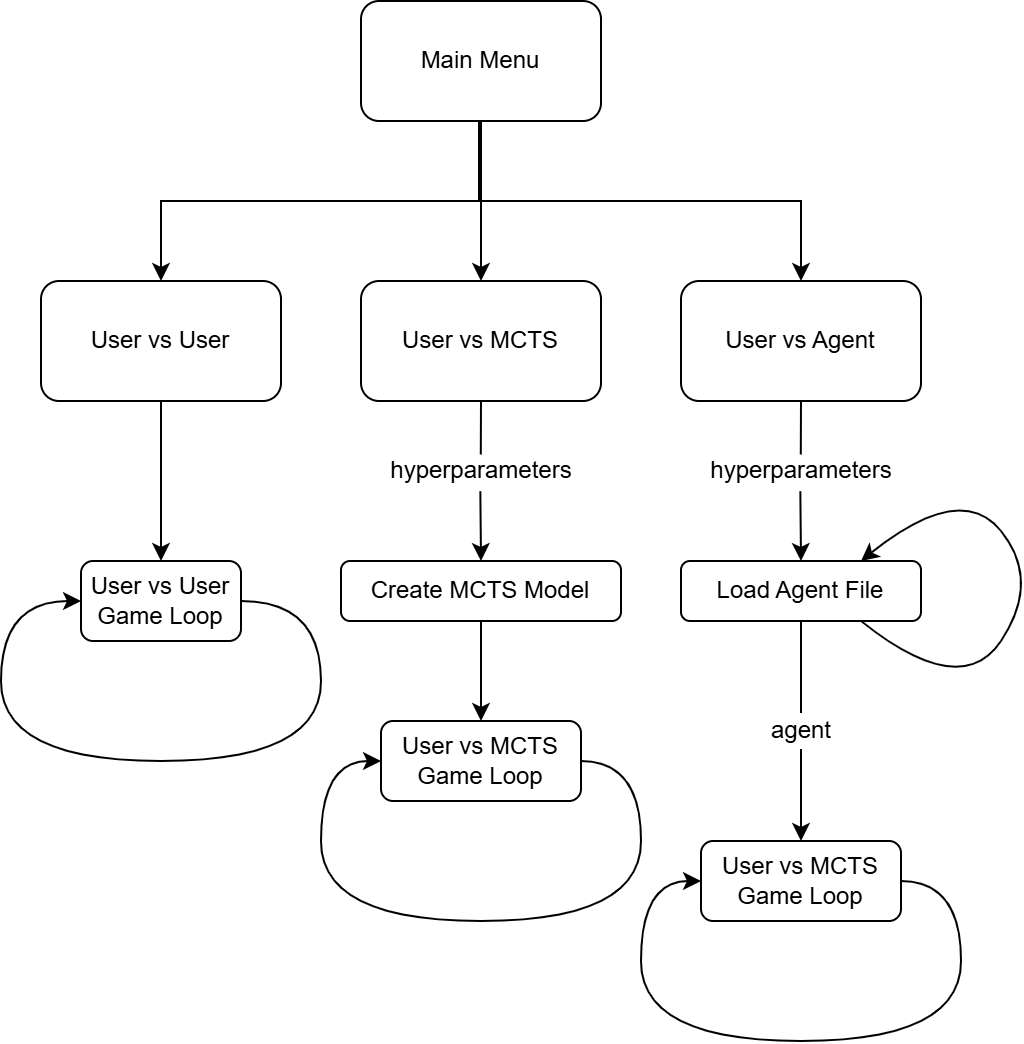
\includegraphics[scale=0.2]{MainMenuHierachyChart.drawio.png}
        \caption{Hierarchy chart for the User Interface}
    \end{figure}

    When the user interface is first shown, it displays the main menu. As seen in the most recent section, the main menu will allow
    users to select various hyperparameters for both the MCTS and complete agent models and then allow the user to begin playing a game of checkers against
    the desired model. For MCTS, the model will be instantiated inside of the program, and a tree build will be run on each turn of the MCTS. For the agent objects,
    its instantiation will be stored inside of a respectively named pickle file - see \myhy{File-Structure}{2.1} - and then loaded into the program.
    
    \subsection{Autodifferentiation Engine}

    The autodifferentiation engine is based mainly around one class - the 'Tensor' class. This class replicates types such as floats, integers, and matrices while adding functionality
    for automatic differentiation of operations on these types. 

    \subsubsection{Data Structures}

    \begin{center}
        \begin{tabular}{|m{10em} | m{12em} | m{15em}|}
            \hline 
                Item & Data Structure & Reasoning and Usage \\
            \hline
            \hline
                Tensor Data & 2D Array & Can represent floats, ints and matrices - with a scalar just being a 1x1 matrix. \\
            \hline
                Tensor Sape & tuple[int,...] & Represents the shape of the data matrix. Useful for iterating through data. \\
            \hline
                Tensor Children + Parents & list[Tensor] & Allows us to store the tensors used to create and created by the given tensor - which then builds the function graph. (see \myhy{Autodiff-example}{example}) \\
            \hline
                Tensor Function Graph & Graph & Represents a graph of operations upon or between input tensors, intermediary tensors, and a final output of a composition of operations. Allows for
                backward traversal and therefore computation of partial derivatives of the output with respect to its inputs. \\
            \hline
        \end{tabular}
    \end{center}

    \subsubsection{Algorithms}

    The key algorithms for this module include the depth first search backwards through the function graph and various algorithms relating to convolution
    and correlation operations on matrices, and their derivatives. Some smaller processes include the removing of extra dimensions which are a result of numpys broadcasting.
    Psuedocode for the backward traversal through the computational graph has been seen in the analysis section - \myhy{Analysis-IoA}{here}.

    \subsubsubsection{Unbroadcasting}  
    The numpy library broadcasts dimensions to allow for vector multiplication which is more efficient than iteration.
    Using an example where we must remove broadcasted dimensions, say we have a matrix $a$, and its shape is $3 \times 1 \times 4$ and its initially computed
    gradient ($da$) has shape $5 \times 3 \times 2 \times 4$ after any broadcasting. We must first sum out any added dimensions using the algorithm below.

    \begin{algorithm} 
        \caption{Sum Added Dims}
        \begin{algorithmic}
        \Function{SumAddedDims}{Array a, Array da}
            \State numInDims $\gets$ len(a.shape)
            \State numGradDims $\gets$ len(da.shape)

            \For {n in range(numGradDims - numInDims)} \Comment{This would result in 1 loop}
                \State da $\gets$ da.sum() \Comment{This would sum out the first dimension leaving da as $3 \times 1 \times 4$}
            \EndFor
        \EndFunction
        \end{algorithmic}
    \end{algorithm}

    \pagebreak
    The next step is to reduce any broadcasted dimensions back to singular dimensions. To do this we can use the below algorithm.

    \begin{algorithm} 
        \caption{Sum Broadcasted Dims}
        \begin{algorithmic}
        \Function{SumBroadcastedDims}{Array a, Array da}
            \For {dim in a.shape} \Comment{a.shape would be equal to (3,1,4)}
                \If {dim == 1}
                    \State da $\gets$ da.sum(axis=dim, keepdims=True)
                \EndIf 
            \EndFor
        \EndFunction
        \end{algorithmic}
    \end{algorithm}

    Note here that we pass in the axis we want to sum across and we set 'keepdims' equal to true. Since we have removed the added dimensions using the previous
    algorithm, we now want to keep the number of dimensions the same. 'keepdims' does this by making the summed axis reduce to 1. So after both
    of these algorithms $da$ would have the same shape as $a$ - which is exactly what we want!
    
    \subsubsubsection{Cross-Correlation, Convolution and derivatives}
    The valid cross-correlation of 2D matrices has been mentioned and demonstrated in the analysis (\myhy{Analysis-MathematicalFormulae}{Mathematical Formulae}), but in the design I will provide a visual representation of
    this process. To put it into writing again, imagine an input matrix of size $(x \times x)$ and a second 'kernel' of size $(k \times k)$. The output of a cross-correlation between these matrices will have a size
    of $(y \times y), y = x - k + 1$. To compute the output, place the kernel ontop of the input so that the top left corners line up, and sum the products of the overlying elements. This number will givee the result
    for the first element of the output matrix. Slide the kernel over and repeat to process, giving the second element of the output. And repeat until the ouput matrix is full.

    \begin{figure}[h]
        \centering
        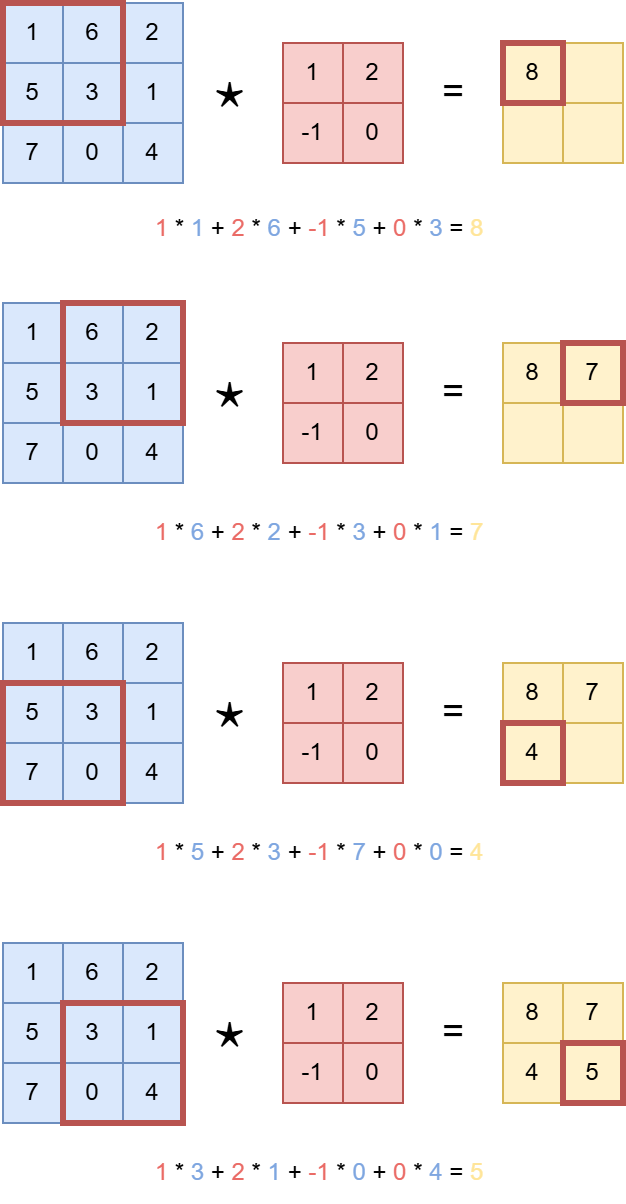
\includegraphics[scale=0.275]{Cross-Correlation-Algorithm.drawio.png}
        \caption{Valid Cross-Correlation Visualization}
    \end{figure}
    
    The above operation is used in the forward pass of a convolutional layer and its derivative includes a variation of the below version of cross-correlation. 
    As also mentioned in the analysis section, there is another form of cross-correlation called 'full' cross-correlation, and the first few steps of the 
    process for this full cross-correlation can be seen below.

    \begin{figure}[h]
        \centering
        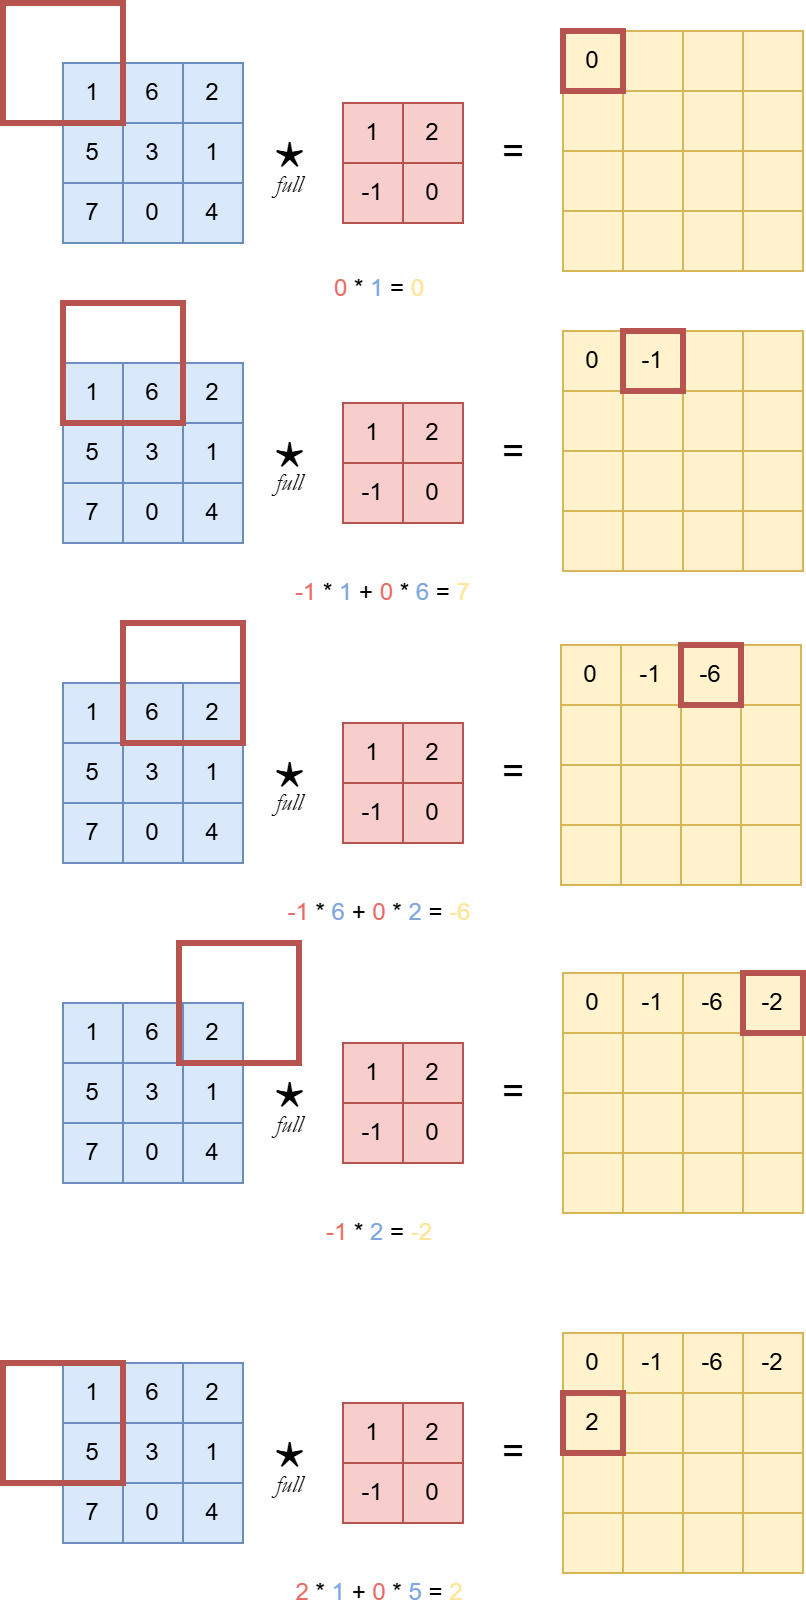
\includegraphics[scale=0.275]{Full-Cross_Correlation-Algorithm.drawio.png}
        \caption{Initial Steps of a Full Cross-Correlation Visualization}
    \end{figure}
    
    To then complete whats known as a convolution, you would complete the cross-correlation but rotate the kernel 180 degrees. This works for both version of cross-correlation i.e.
    a full convolution is the same as a full cross-correlation with a rotated kernel and a valid convolution is the same as a valid cross-correlation with a rotated kernel. 

    \subsubsubsection{Tensor Forward and Backward Pass}
    This section will contain a visualization and paired explanation of how a set of operations on a tensor would be completed and then what would happen if we called
    the backward function on the final output tensor. 

    Firstly, say we have tensors $a,b,c$ with values $1,2$ and $3$ respectively. We then define tensors $d,e$ with values $a \times b$ and  $b \times c$ respectively, and finally
    we define our output tensor $y$ with a value of $d \times e$.

    This set of definitions and operations would produce a computational graph of that shown in Figure 22.

    \begin{wrapfigure}[15]{r}{0.52\linewidth}
        \centering
        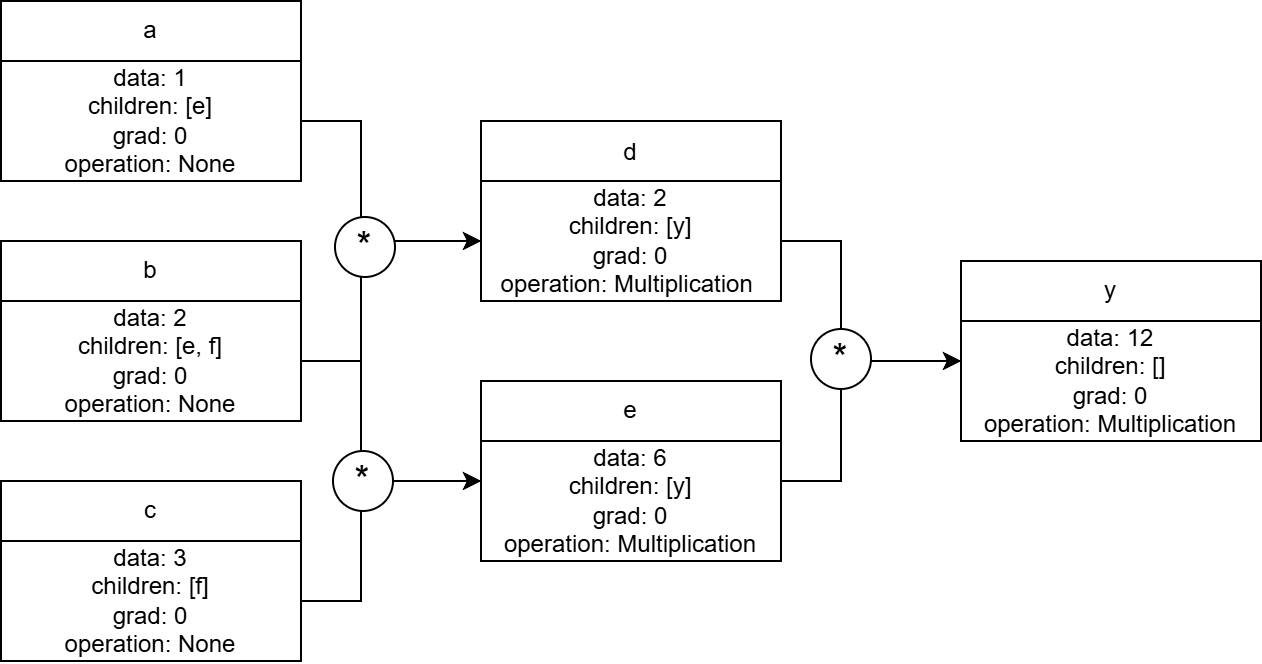
\includegraphics[scale=0.2]{Tensor-forward-example.drawio.png}
        \caption{Computational graph for a given example}
    \end{wrapfigure}

    If we then called the backward function from the output tensor $y$. It would first set the gradient of $y$ to 1, as the gradient of a variable with respect to itself is 1.
    Next it would call the backward function on the instance of the operation class attached to that tensor. So for $y$ this would call the backward function on the specific instance
    on the multiplication operation attached to $y$. Assuming all of these tensors have the 'requires\_grad' variable set to true, this backward function of this multiplication instance would
    calculate the gradients for tensor $d$ (using processes and formulae defined \myhy{Analysis-MathematicalFormulae}{here} and \myhy{Autodiff-example}{here} respectively) and then call backward on that tensor. After the backward of function of $d$ is then completed our function would return to being inside the 
    backward function of the multiplication instance associated with tensor $y$ (seen by the red arrowhead in the tensor $y$ of the diagram below).

    \begin{figure}[h]
        \centering
        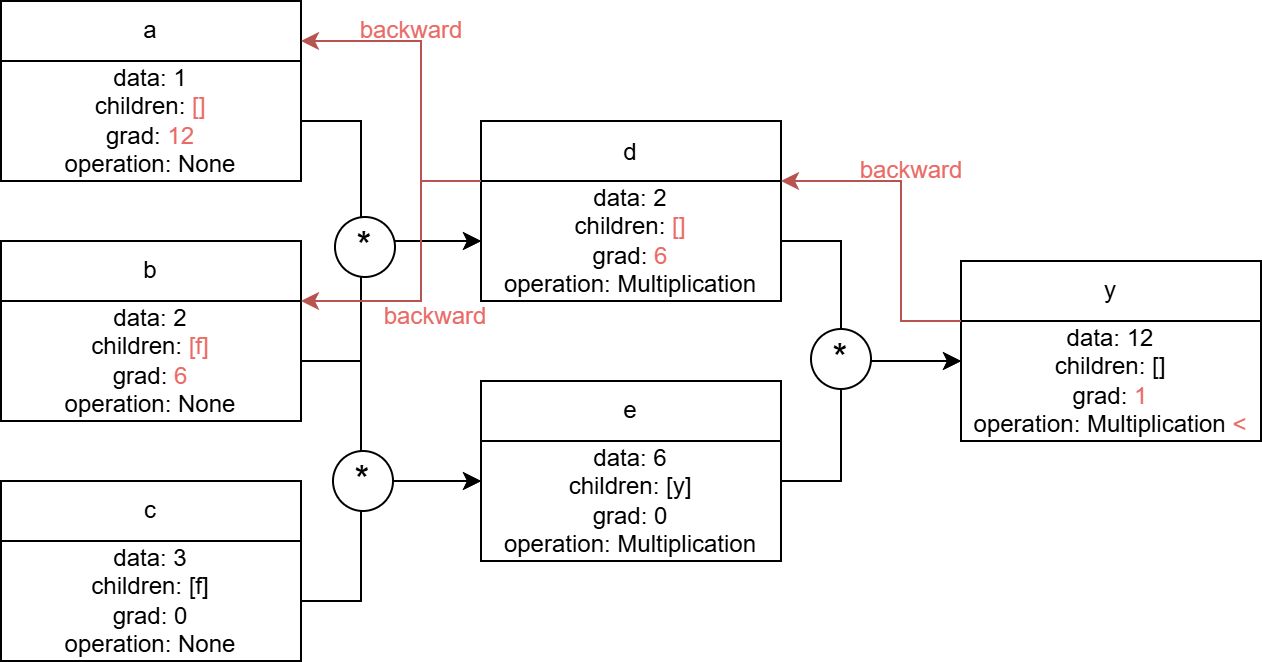
\includegraphics[scale=0.2]{Tensor-backward1-example.drawio.png}
        \caption{Part-way through a backward pass of a computational graph for a given example}
    \end{figure}

    Now, the same process occurs that happened for tensor $d$, but for tensor $e$. Leaving the computational graph in its final, and complete, state as follows:

    \begin{figure}[h]
        \centering
        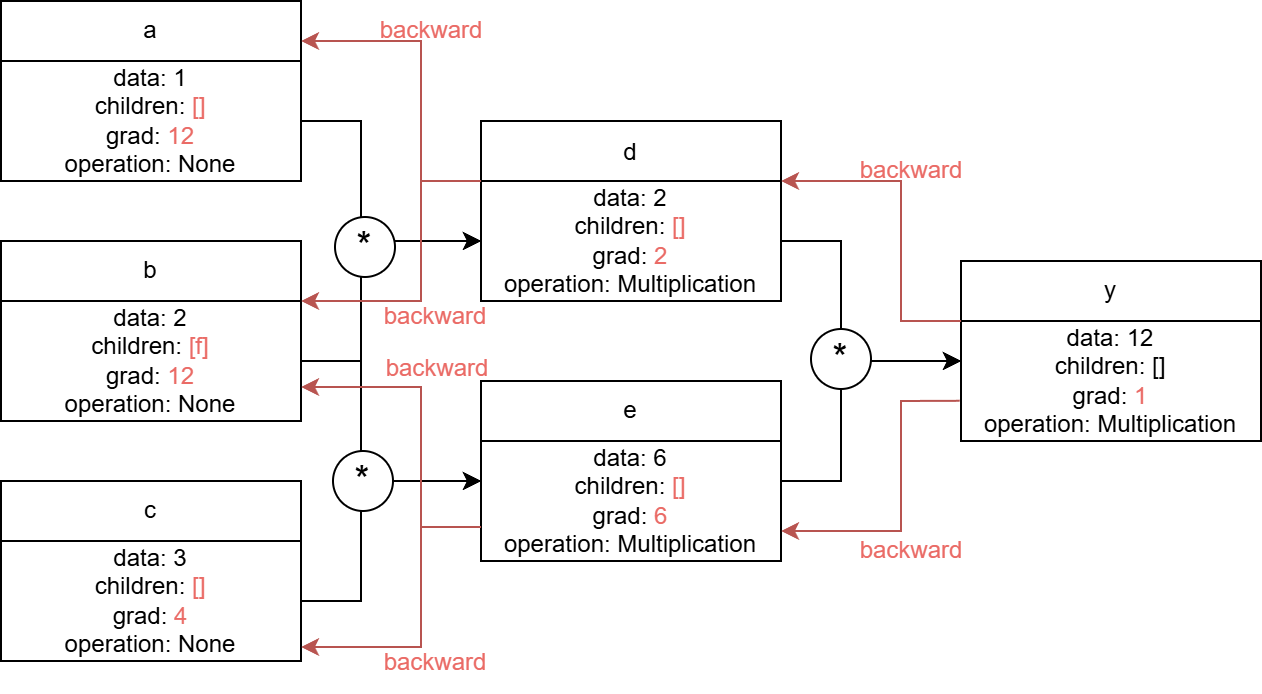
\includegraphics[scale=0.2]{Tensor-backward2-example.drawio.png}
        \caption{Final state after a backward pass of a computational graph for a given example}
    \end{figure}

    \pagebreak
    \subsection{Neural Network Library}

    The neural network library is also based manily around one class, in this case it is the 'Module' Class. 

    \subsubsection{Data Structures}

    The module class is actually an abstract class that provides an interface for different layers and collections of layers.
    It has a property called 'params' which fetches all of the parameters and tensors that compose that module. This is used by optimizers to
    update parameter values. Forward is a basic method which takes an input tensor and then applies any operations defined in the specific
    module, returning the output. Save and load allow the parametes of a module to be saved and loaded using pickle. A module list is similar to a module,
    as it inherits from module, but is also composed of modules. The main difference is inside of the params property as it loops through each
    module it is composed of to fetch its parameters. This is useful for creating a block of similar modules.

    \begin{figure}[h]
        \centering
        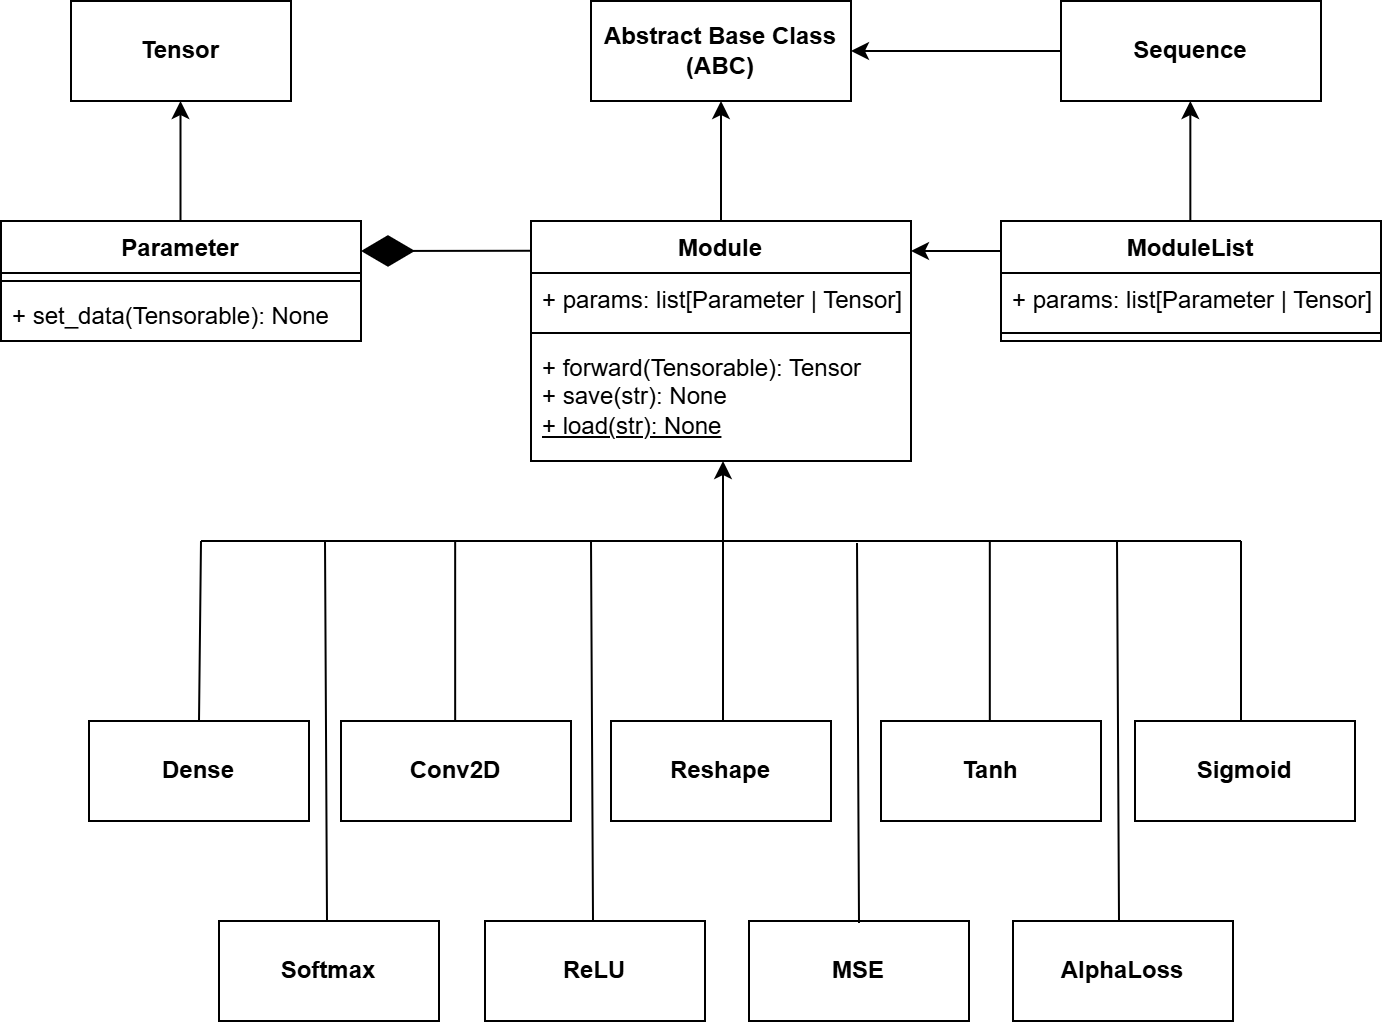
\includegraphics[scale=0.23]{NNLib-Design-UML.drawio.png}
        \caption{Neural Network Library Modules UML}
    \end{figure}

    Another, much smaller, element of the library is the optimizer. This library only implements Stochastic Gradient Descent
    (SGD) but there are many other optimizing models such as Adam and RMSProp. The abstract optimizer class has methods which update
    the value of each parameter using their gradients, the learning rate and the regularization (the step method). As well as a method to
    set all gradients back to 0 - as gradients accumulate with each tensor backward call, they must be reset for each backpropogation.

    \begin{figure}[h]
        \centering
        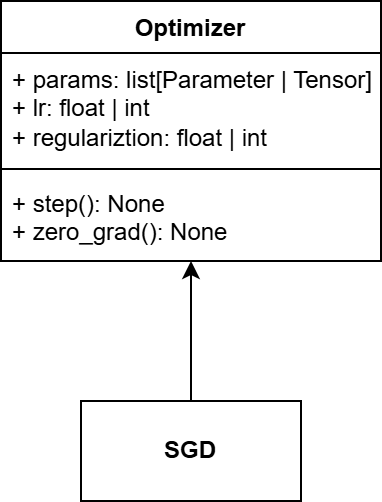
\includegraphics[scale=0.22]{NN-Optimizers-Design-UML.drawio.png}
        \caption{Neural Network Library Optimizers UML}
    \end{figure}

    \pagebreak
    \subsubsection{Algorithms}
    Three of the four key algorithms inside of the neural network library have been mentioned inside of the data structures section; the 'step',
    'zero_grad' and 'params' functions, and pseudocode for those can be seen below.

    \begin{algorithm} 
        \caption{Optimizer Step Function}
        \begin{algorithmic}
        \Function{Step}{Optimzier self}
            \For {param in self.params}
                \State param.data $\gets$ param.data - self.lr * (param.grad - self.regularization * (param.data ** 2))
            \EndFor
        \EndFunction
        \end{algorithmic}
    \end{algorithm}

    This simple function completes the small steps towards a more optimal parameter value - as explained \myhy{Analysis-GradientDescent}{here} in the analysis and
    is therefore crucial to the library, and the learning process for modules.

    \begin{algorithm} 
        \caption{Optimizer Zero Grad Function}
        \begin{algorithmic}
        \Function{ZeroGrad}{Optimzier self}
            \For {param in self.params}
                \State param.grad $\gets$ 0
            \EndFor
        \EndFunction
        \end{algorithmic}
    \end{algorithm}

    Again, a simple but crucial function. As gradient accumulates, if the gradients are not reset after each training iteration, the values from past iterations
    may skew the step process and therefore inhibit learning.

    \begin{algorithm} 
        \caption{Module Params Property Definition}
        \begin{algorithmic}
        \Function{Params}{Module self}
            \State params $\gets$ []
            \For {param in self.attributes}
                \If{param is Module or ModuleList}
                    \State params += param.params
                \ElsIf{param is Parameter}
                    \State params.append(param)
                \ElsIf{param is Tensor and param.requires_grad}
                    \State params.append(param)
                \EndIf
            \EndFor
        \EndFunction
        \end{algorithmic}
    \end{algorithm}

    The params function gets all values associated with a module or module list that are 'trainable parameters'. This means
    any values which need to get updated during the step process. This property also uses recursion to add parameters from a module
    which has another module inside of itself.


    \begin{wrapfigure}[8]{r}{0.7\linewidth}
        \centering
        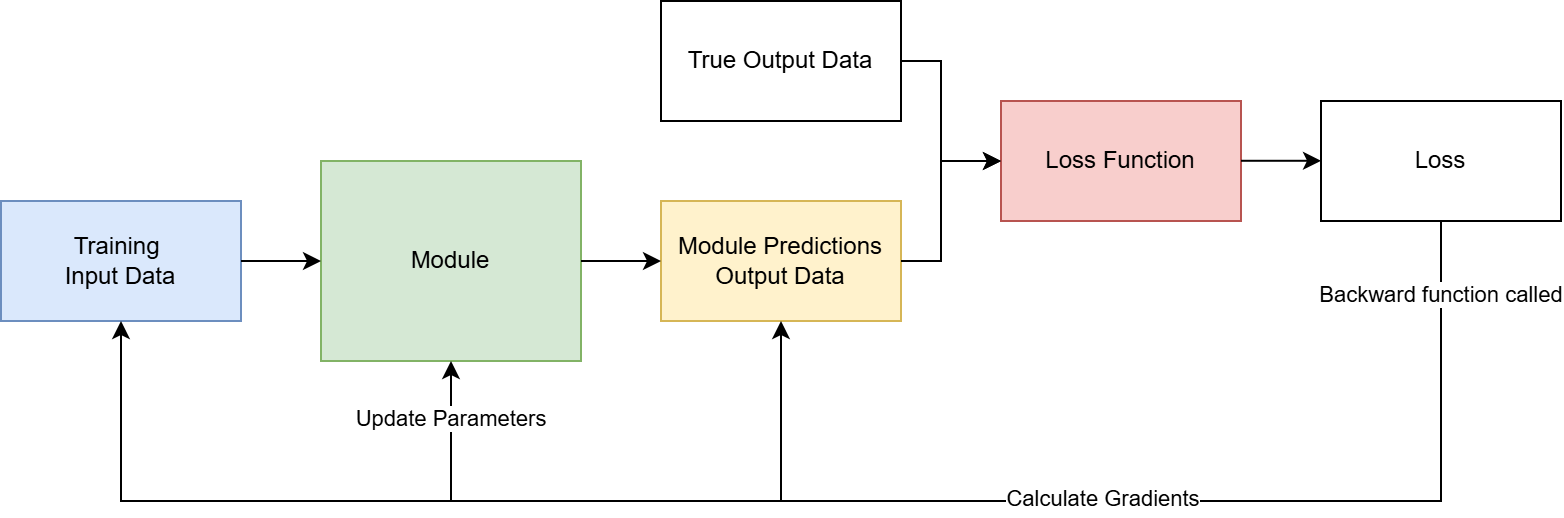
\includegraphics[scale=0.2]{ModuleTrainingFlow.drawio.png}
        \caption{Neural Network Library Modules UML}
    \end{wrapfigure}

    The final key algorithm is the general approach to training a module. This was defined in the analysis and psuedocode can be
    seen \myhy{Analysis-IofA-NNLib}{in this section}. 
    
    \vspace{1mm}
    To the right, there is also a visualization of one iteration of
    this learning process.
    

    \pagebreak
    \subsection{Reinforcement Learning Solution}
    The reinforcement learning section is the most complex of all the parts. It uses all the classes and builds the learning agent
    from all the tools defined, and ones that will be defined in this section. The final product is a model that can play checkers at
    a higher level with the same or less time, than a tree search.
    \subsubsection{Data Structures}

    \subsubsection{Algorithms}

    \subsubsection{Structure, Hierarchy and Flow}

    \subsubsection{Non-standard Design}

    \begin{figure}
        \centering
        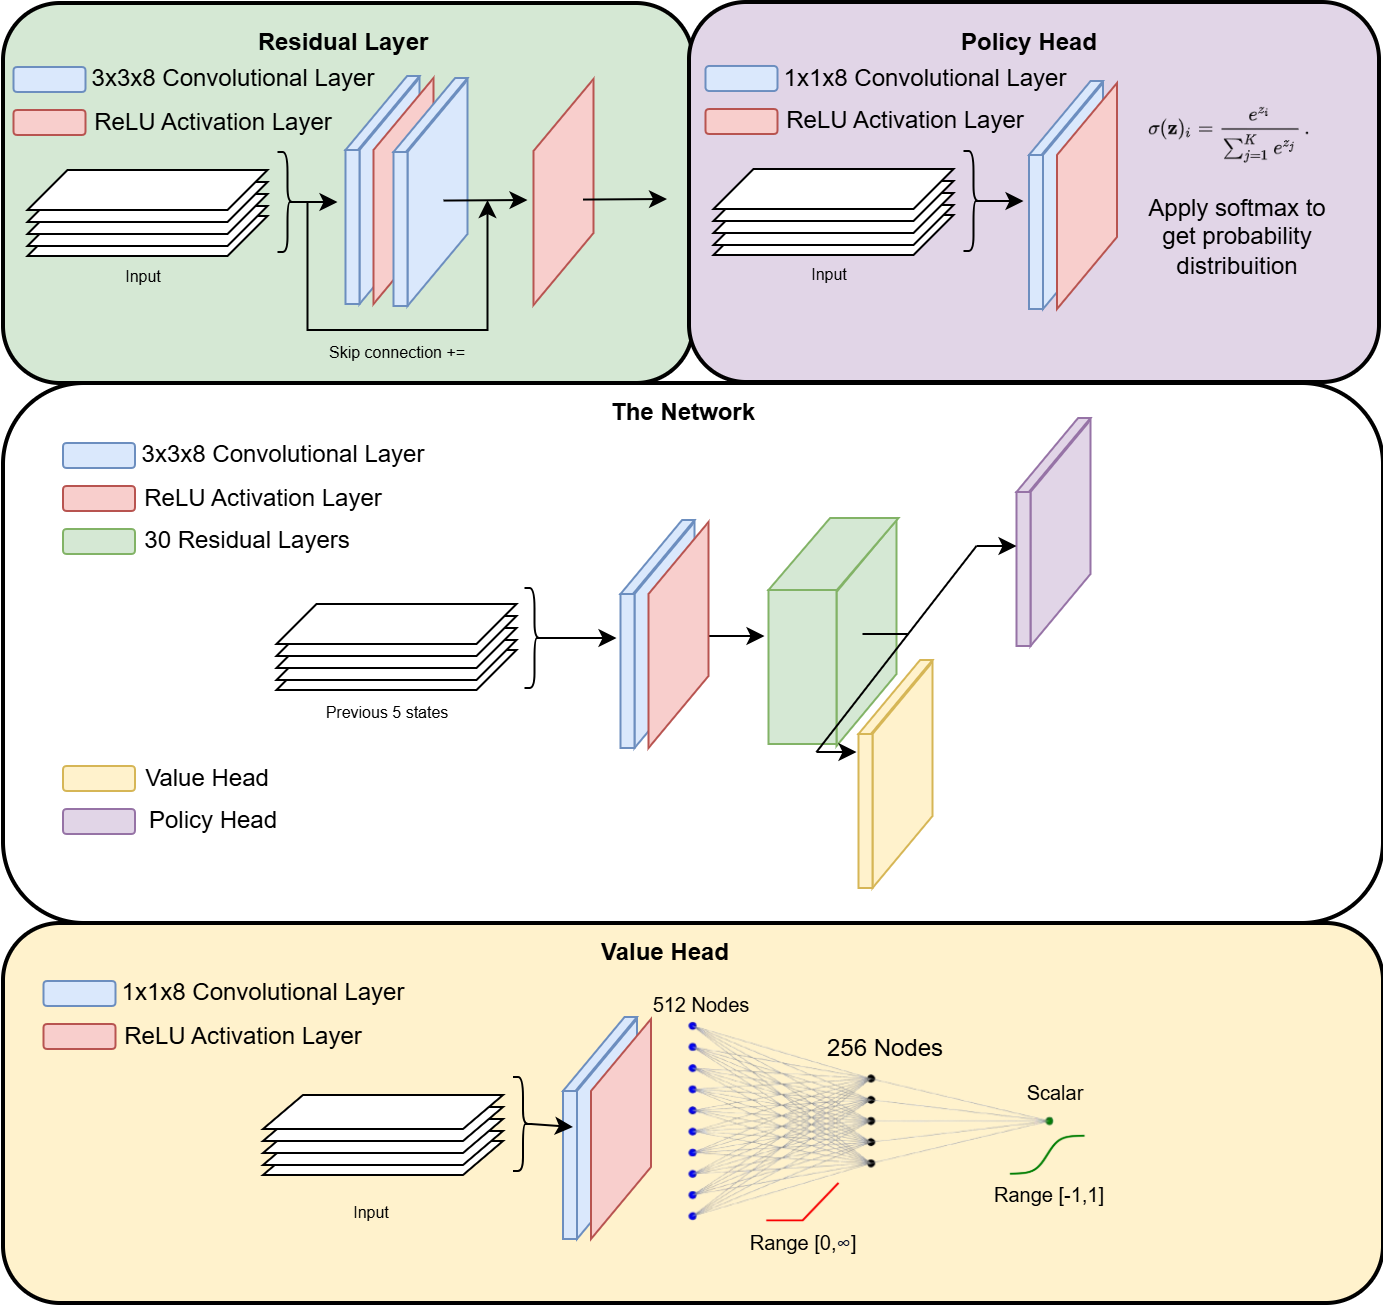
\includegraphics[scale=0.45]{NetworkPassThrough.drawio.png}
        \caption{A representation of the AlphaNetwork}
    \end{figure}

    
    \pagebreak
    \section{Research Log}

    \subsection{Checkers}
    \subsubsection{Rules}
    \noindent \url{https://www.mastersofgames.com/rules/checkers-rules.htm}
    \subsubsection{Possible States}
    \noindent \url{https://math.stackexchange.com/questions/2240519/how-to-find-the-amount-of-possible-piece-configurations-in-the-game-of-checkers}
    
    \subsection{Neural Networks}
    \noindent \url{https://www.ibm.com/topics/neural-networks}

    \subsubsection{Vectorization of summations}
    \noindent \url{https://courses.cs.washington.edu/courses/cse446/20wi/Lecture8/08_Regularization.pdf}

    \subsubsection{Convolutional Networks}
    \noindent \url{https://www.youtube.com/watch?v=Lakz2MoHy6o}\\

    \subsection{Automatic Differentiation}
    \noindent \url{https://en.wikipedia.org/wiki/Automatic_differentiation}

    \subsection{AlphaZero}
    \noindent \url{https://ai.stackexchange.com/questions/13156/does-alphazero-use-q-learning}
    \noindent \url{https://suragnair.github.io/posts/alphazero.html}
    Explanations of AlphaZero's loss function
    \noindent \url{https://www.davidsilver.uk/wp-content/uploads/2020/03/unformatted_final_mastering_go.pdf} Methods and Neural Network architecture section

    \noindent \url{https://liacs.leidenuniv.nl/~plaata1/papers/CoG2019.pdf}
    AlphaZero policy explanation

    \subsection{Existing Auto differentiation systems}
    \noindent \url{https://medium.com/@utsavstha/jax-vs-pytorch-a-comprehensive-comparison-for-deep-learning-10a84f934e17}
    PyTorch vs JAX

    \subsection{Reinforcement Learning}
    \noindent \url{https://web.stanford.edu/class/psych209/Readings/SuttonBartoIPRLBook2ndEd.pdf} What is reinforcement learning?\\
    \noindent \url{https://smartlabai.medium.com/reinforcement-learning-algorithms-an-intuitive-overview-904e2dff5bbc} Intro to reinforcement learning\\
    \noindent \url{https://medium.com/the-official-integrate-ai-blog/understanding-reinforcement-learning-93d4e34e5698} Different types of reinforcement learning\\
    \noindent \url{https://neptune.ai/blog/model-based-and-model-free-reinforcement-learning-pytennis-case-study} Model-based vs Model-free learning\\
\end{document}